\documentclass[a4paper,12pt]{article}
\usepackage{docsTemplate}
\usepackage{array}
\usepackage{longtable}
\usepackage{float}
\usepackage[official]{eurosym}
\usepackage{pgf-pie}
\usepackage{makecell}
\usepackage{xltabular}
\usepackage{amsmath}
\usepackage{caption}
\setcounter{secnumdepth}{4}
\setcounter{tocdepth}{4}
\setTitle{Specifica Tecnica}
\setAuthors{Mattia Oliva Medin \\ & Francesco Balestro \\ & Bianca Zaghetto}
\setVerificators{Nenad Radulovic \\ & Filippo Compagno \\ & Francesco Balestro \\ & Bianca Zaghetto \\ & Sara Gioia Fichera}
\setApprovation{}
\setVersion{0.5}
\setType{Esterno}
\setDestination{Team Three Technologies \\ & Prof. Tullio Vardanega \\ & Prof. Riccardo Cardin \\ & Sanmarco Informatica SpA}

\begin{document}
    \include{docTitlepage}

    \section*{Registro delle modifiche} {
        \begin{table}[h!]
            \rowcolors{2}{lightgray}{white}
                \begin{tabularx}{\textwidth}{|l|l|l|l|L|L|}
                \hline
                \textbf{Vers.} & \textbf{Data} & \textbf{Autore} & \textbf{Ruolo} & \textbf{Verifica} & \textbf{Oggetto} \\
                \hline
                \textbf{0.5} & 25/04/26 & Francesco Balestro & Programmatore & Bianca Zaghetto & Prima stesura "Design pattern", "Oggetti di trasferimento dati", "Presentation layer" e "Application layer" \\
                \hline
                \textbf{0.4} & 22/04/26 & Francesco Balestro & Responsabile & Sara Gioia Fichera & Prima stesura Architetture e aggiornamento sezione "Tecnologie" \\
                \hline
                \textbf{0.3} & 14/04/26 & Bianca Zaghetto & Programmatore & Francesco Balestro & Riferimenti normativi \\
                \hline
                \textbf{0.2} & 13/04/26 & Francesco Balestro & Verificatore & Filippo Compagno & Sezione "Scopo del documento" e "Tecnologie" \\
                \hline
                \textbf{0.1} & 11/04/26 & Mattia Oliva Medin & Programmatore & Nenad Radulovic & Prima stesura \\
                \hline
            \end{tabularx}
        \end{table}
    }
    \newpage
    
    \tableofcontents
    \newpage

    \listoffigures
    \newpage
    
    \listoftables
    \newpage

    \section{Introduzione} {
        \subsection{Scopo del documento} {        
            Il presente documento ha lo scopo di descrivere in maniera approfondita l’architettura del prodotto software, offrendo una rappresentazione chiara, organizzata e completa delle sue componenti, delle modalità con cui interagiscono e della loro distribuzione all’interno del sistema.\\
            \\
            La Specifica Tecnica costituisce un riferimento fondamentale per le attività di progettazione e sviluppo del prodotto, introducendo evoluzioni e miglioramenti volti a rafforzarne la solidità architetturale rispetto al PoC.\\
            \\
            In particolare, questo documento si propone di:
            \begin{itemize}
                \item Definire l’architettura logica del sistema, descrivendo le componenti principali, le rispettive responsabilità e le relazioni tra esse;
                \item Illustrare l’architettura di deployment, specificando come le diverse componenti vengono distribuite nell’ambiente di esecuzione;
                \item Presentare i design pattern architetturali adottati, mettendo in evidenza le scelte progettuali legate alle tecnologie utilizzate;
                \item Fornire ulteriori dettagli progettuali utili a valorizzare le decisioni architetturali e a facilitare la comprensione e la manutenzione del sistema.
            \end{itemize}
        }

        \subsection{Glossario} {
            Si rimanda al documento Glossario per chiarire i termini nel dominio del progetto che possono risultare ambigui o di difficile comprensione. I vocaboli presenti nel glossario sono stati segnalati seguendo la notazione:
            \begin{center}
                parola\textsubscript{G}
            \end{center}
        }
        
        \subsection{Riferimenti} {
            \subsubsection{Riferimenti normativi} {
                \begin{itemize}
                    \item \textit{Norme di progetto v1.0}
                    \begin{itemize}
                        \item \url{https://team-three-technologies.github.io/Documenti/2%20-%20PB/Documenti%20Interni/Norme_di_Progetto_v1_0.pdf}
                        \item[] (Ultimo accesso: 2026/04/11)
                    \end{itemize}
                    \item Capitolato C3
                    \begin{itemize}
                        \item \url{https://www.math.unipd.it/~tullio/IS-1/2025/Progetto/C3.pdf}
                        \item[] (Ultimo accesso: 2026/01/11)
                    \end{itemize}
                    \item Regolamento del Progetto Didattico
                    \begin{itemize}
                        \item \url{https://www.math.unipd.it/~tullio/IS-1/2025/Dispense/PD1.pdf}
                        \item[] (Ultimo accesso: 2026/04/05)
                    \end{itemize}
                \end{itemize}
            }
            \subsubsection{Riferimenti informativi} {
                \begin{itemize}
                    \item \textit{Glossario v0.5}
                    \begin{itemize}
                        \item \url{https://team-three-technologies.github.io/Documenti/1%20-%20RTB/Documenti%20interni/Glossario_v0_5.pdf}
                        \item[] (Ultimo accesso: 2026/MM/DD)
                    \end{itemize}
                \end{itemize}
            }
        }
    }

    \section{Tecnologie} {
        Il progetto è stato realizzato adottando un insieme di tecnologie consolidate e complementari, selezionate per garantire semplicità di sviluppo, portabilità e facilità di manutenzione, in linea con un’architettura di tipo monolitico.\\
        \\
        La soluzione prevede un’applicazione desktop sviluppata utilizzando Angular per la gestione dell’interfaccia utente, integrata con Electron per la creazione del pacchetto eseguibile e per l’esecuzione in ambiente desktop. La comunicazione tra le componenti avviene tramite meccanismi di Inter-Process Communication (IPC) messi a disposizione da Electron, consentendo un’interazione strutturata ed efficiente tra le diverse parti dell’applicazione.\\
        \\
        Per la gestione della persistenza dei dati è stato adottato SQLite, scelto per la sua leggerezza, semplicità di integrazione e adeguatezza a contesti applicativi locali. In particolare, il database viene utilizzato per memorizzare e gestire i dati relativi al DIP, permettendone la consultazione e la visualizzazione all’interno dell’applicazione.\\
        \\
        Le tecnologie adottate sono state classificate in funzione del loro ruolo architetturale all’interno del sistema, includendo linguaggi di programmazione, framework per lo sviluppo dell’interfaccia utente, framework e runtime per l’esecuzione e il packaging dell’applicazione desktop, meccanismi di comunicazione tra componenti e sistemi di persistenza dei dati.\\
        \\
        Di seguito vengono descritte nel dettaglio le tecnologie adottate, evidenziandone le caratteristiche principali.

        \subsection{Linguaggi di Programmazione}
        \begin{table}[H]
            \captionsetup{skip=10pt}
            \caption{Linguaggi di Programmazione}
            \rowcolors{1}{lightgray}{white}
            \begin{tabular}{|>{\centering\arraybackslash}m{0.20\linewidth}|>{\centering\arraybackslash}m{0.10\linewidth}|>{\centering\arraybackslash}m{0.62\linewidth}|}
                \hline
                \textbf{Tecnologia} & \textbf{Versione} & \textbf{Descrizione} \\
                \hline
                \textbf{TypeScript} & 5.9.3 & TypeScript è un linguaggio di programmazione tipizzato basato su JavaScript, utilizzato per migliorare la qualità del codice grazie alla tipizzazione statica e al supporto per lo sviluppo di applicazioni scalabili e manutenibili. \\
                \hline
            \end{tabular}
        \end{table}

        \subsection{Framework per lo sviluppo dell'interfaccia utente}
        \begin{table}[H]
            \captionsetup{skip=10pt}
            \caption{Framework per lo sviluppo dell'interfaccia utente}
            \rowcolors{1}{lightgray}{white}
            \begin{tabular}{|>{\centering\arraybackslash}m{0.20\linewidth}|>{\centering\arraybackslash}m{0.10\linewidth}|>{\centering\arraybackslash}m{0.62\linewidth}|}
                \hline
                \textbf{Tecnologia} & \textbf{Versione} & \textbf{Descrizione} \\
                \hline
                \textbf{Angular} & 21.2.0 & Angular è un framework frontend basato su TypeScript, utilizzato per la realizzazione di applicazioni web strutturate e modulari tramite un’architettura a componenti. \\
                \hline
            \end{tabular}
        \end{table}

        \subsection{Framework e runtime di esecuzione desktop}
        \begin{table}[H]
            \captionsetup{skip=10pt}
            \caption{Framework e runtime di esecuzione desktop}
            \rowcolors{1}{lightgray}{white}
            \begin{tabular}{|>{\centering\arraybackslash}m{0.20\linewidth}|>{\centering\arraybackslash}m{0.10\linewidth}|>{\centering\arraybackslash}m{0.62\linewidth}|}
                \hline
                \textbf{Tecnologia} & \textbf{Versione} & \textbf{Descrizione} \\
                \hline
                \textbf{Electron} & 40.8.2 & Electron è un framework per lo sviluppo di applicazioni desktop multipiattaforma basato su tecnologie web, che integra un runtime basato su Chromium e Node.js e fornisce strumenti per il packaging e l’esecuzione dell’applicazione. \\
                \hline
            \end{tabular}
        \end{table}

        \subsection{Librerie}
        \begin{table}[H]
            \captionsetup{skip=10pt}
            \caption{Librerie}
            \rowcolors{1}{lightgray}{white}
            \begin{tabular}{|>{\centering\arraybackslash}m{0.20\linewidth}|>{\centering\arraybackslash}m{0.10\linewidth}|>{\centering\arraybackslash}m{0.62\linewidth}|}
                \hline
                \textbf{Tecnologia} & \textbf{Versione} & \textbf{Descrizione} \\
                \hline
                \textbf{ngx-doc-viewer} & 21.0.5 & Libreria Angular per la visualizzazione di documenti direttamente nel browser tramite viewer integrati. \\
                \hline
                \textbf{better-sqlite3} & 12.6.2 & Libreria per Node.js che fornisce un’interfaccia sincrona ed efficiente per l’utilizzo di database SQLite, integrando direttamente il motore SQLite e semplificando l’esecuzione di query e la gestione dei dati. \\
                \hline
                \textbf{fast-xml-parser} & 5.5.9 & Libreria JavaScript veloce per il parsing e la conversione di file XML in oggetti JavaScript, e viceversa. \\
                \hline
                \textbf{tsyringe} & 4.10.0 & Libreria di dependency injection per TypeScript che facilita la gestione delle dipendenze e l’inversione del controllo. \\
                \hline
            \end{tabular}
        \end{table}

        \subsection{Strumenti di sviluppo}
        \begin{table}[H]
            \captionsetup{skip=10pt}
            \caption{Strumenti di sviluppo}
            \rowcolors{1}{lightgray}{white}
            \begin{tabular}{|>{\centering\arraybackslash}m{0.20\linewidth}|>{\centering\arraybackslash}m{0.10\linewidth}|>{\centering\arraybackslash}m{0.62\linewidth}|}
                \hline
                \textbf{Tecnologia} & \textbf{Versione} & \textbf{Descrizione} \\
                \hline
                \textbf{prettier} & 3.8.1 & Prettier è un formatter automatico di codice che garantisce uno stile consistente e leggibile in diversi linguaggi. \\
                \hline
                \textbf{electron-builder} & 26.8.1 & Strumento per il packaging e la distribuzione di applicazioni Electron in eseguibili per diverse piattaforme. \\
                \hline
            \end{tabular}
        \end{table}

        \subsection{Tecnologie per analisi dinamica}
        \begin{table}[H]
            \captionsetup{skip=10pt}
            \caption{Tecnologie per analisi dinamica}
            \rowcolors{1}{lightgray}{white}
            \begin{tabular}{|>{\centering\arraybackslash}m{0.20\linewidth}|>{\centering\arraybackslash}m{0.10\linewidth}|>{\centering\arraybackslash}m{0.62\linewidth}|}
                \hline
                \textbf{Tecnologia} & \textbf{Versione} & \textbf{Descrizione} \\
                \hline
                \textbf{vitest} & 4.0.8 & Vitest è un framework di testing veloce per progetti JavaScript/TypeScript, progettato per integrarsi con Vite e supportare test unitari e di integrazione. \\
                \hline
                \textbf{@vitest/coverage-v8} & 4.0.8 & @vitest/coverage-v8 è un plugin per Vitest che utilizza il motore V8 per generare report di code coverage durante l’esecuzione dei test. \\
                \hline
            \end{tabular}
        \end{table}
    }

    \section{Architettura} {
        \subsection{Architettura logica} {
            Il sistema è progettato seguendo un’\textbf{architettura layered}, che organizza l’applicazione in livelli distinti con responsabilità ben definite, al fine di garantire una chiara separazione delle competenze, una maggiore manutenibilità e una migliore scalabilità logica del sistema.\\
            \\
            In questo modello architetturale, ogni livello espone servizi ben definiti verso il livello superiore e interagisce esclusivamente con quelli adiacenti, riducendo l’accoppiamento tra le componenti. Questa struttura consente di isolare la logica di presentazione, la logica applicativa e la gestione dei dati, facilitando l’evoluzione indipendente delle singole parti del sistema.\\
            \\
            L’applicazione è organizzata in tre livelli principali: \textit{presentation layer}, \textit{application layer} e \textit{data layer}, ciascuno con un ruolo ben definito all’interno del sistema.
            \begin{itemize}
                \item Il \textbf{presentation layer} è responsabile dell’interfaccia utente e della visualizzazione dei contenuti del DIP (Dissemination Information Package). È implementato tramite \textit{Angular} e gestisce il rendering delle viste, l’interazione con l’utente e la presentazione dei documenti e dei metadati.
                \item L'\textbf{application layer} contiene la logica applicativa e coordina le operazioni tra interfaccia utente e accesso ai dati. È integrato nel contesto di \textit{Electron} e si occupa della gestione del flusso applicativo, della comunicazione tra processi tramite IPC e dell’orchestrazione delle operazioni sul DIP
                \item Il \textbf{data layer} gestisce la persistenza e l’accesso ai dati contenuti nel pacchetto DIP. Utilizza \textit{better-sqlite3} per l’interazione con il database locale, permettendo l’esecuzione di query sui metadati e la gestione strutturata delle informazioni archivistiche.\\
            \end{itemize}
            La comunicazione tra i diversi livelli, in particolare tra presentation layer e application layer, avviene attraverso meccanismi di IPC forniti nativamente da Electron, che permettono un’interazione controllata tra i processi mantenendo una separazione tra interfaccia utente e logica applicativa.
        }
        
        \subsection{Architettura di deployment} {
            L’architettura di deployment del sistema è di tipo \textbf{monolitico}, in quanto l’applicazione viene distribuita come un’unica unità software autocontenuta. Tutte le componenti necessarie al funzionamento del sistema, incluse le dipendenze e le risorse applicative, sono incluse all’interno dello stesso pacchetto installabile.\\
            \\
            Questa scelta consente di semplificare il processo di installazione e configurazione per l’utente finale, eliminando la necessità di servizi esterni o di componenti distribuiti. L’applicazione può quindi essere eseguita in locale in modo indipendente, garantendo portabilità e coerenza dell’ambiente di esecuzione.\\
            \\
            Il packaging e la distribuzione dell’applicazione sono gestiti tramite \textit{electron-builder}, uno strumento specifico per applicazioni \textit{Electron}, che consente la creazione di eseguibili per le principali piattaforme desktop. Questo processo permette di ottenere un unico installer che incapsula l’intero sistema e tutte le sue dipendenze.
        }

        \subsection{Design pattern} {
            \subsubsection{Dependency injection} {
                \paragraph{Descrizione del pattern}\mbox{}\\
                Il pattern Dependency Injection è un design pattern che ha lo scopo di separare la creazione delle dipendenze dall’utilizzo delle stesse all’interno dei componenti di un sistema.\\
                \\
                In questo approccio, un oggetto non istanzia direttamente le proprie dipendenze, ma le riceve dall’esterno, tipicamente tramite il costruttore o metodi dedicati. Questo consente di definire in modo esplicito le relazioni tra i componenti, riducendo l’accoppiamento e migliorando l’organizzazione del codice.\\
                \\
                Le modalità principali attraverso cui può essere applicata la dependency injection sono:
                \begin{itemize}
                    \item Constructor Injection: le dipendenze vengono fornite al momento della creazione dell’oggetto;
                    \item Setter Injection: le dipendenze vengono assegnate successivamente tramite metodi setter.
                \end{itemize}
                
                \noindent Nel contesto del progetto è stato adottato l’approccio basato su Constructor Injection.
                
                \paragraph{Motivazioni dell’utilizzo del pattern}\mbox{}\\
                L’adozione del pattern Dependency Injection all’interno del progetto consente di ottenere diversi benefici:
                \begin{itemize}
                    \item \textbf{riduzione dell’accoppiamento}: i componenti non dipendono direttamente dalle implementazioni concrete delle loro dipendenze;
                    \item \textbf{flessibilità}: è possibile sostituire facilmente le implementazioni senza modificare il codice client;
                    \item \textbf{testabilità}: facilita l’utilizzo di oggetti simulati (mock) durante le fasi di test;
                    \item \textbf{modularità}: i componenti risultano più indipendenti e riutilizzabili;
                    \item \textbf{gestione semplificata delle dipendenze}: consente di delegare la creazione e l’iniezione delle dipendenze a componenti esterni o framework dedicati.
                \end{itemize}
                
                \paragraph{ Utilizzo del pattern nel progetto}\mbox{}\\
                Testo...
            }
            \subsubsection{Builder} {
                \paragraph{Descrizione del pattern}\mbox{}\\
                Il pattern Builder è un design pattern creazionale che consente di costruire oggetti complessi passo dopo passo, separando il processo di costruzione dalla rappresentazione finale dell’oggetto.\\
                \\
                Questo pattern risulta particolarmente utile quando un oggetto deve essere creato con numerosi parametri opzionali o con diverse configurazioni possibili. Il Builder fornisce un’interfaccia fluida per impostare le proprietà desiderate e costruire infine l’oggetto tramite un metodo dedicato.\\
                \\
                Il processo di costruzione avviene tipicamente attraverso una classe builder che espone metodi per impostare i vari attributi e un metodo finale (ad esempio build()) che restituisce l’oggetto completo.
                
                \paragraph{Motivazioni dell’utilizzo del pattern}\mbox{}\\
                L’utilizzo del pattern Builder nel progetto porta i seguenti vantaggi:
                \begin{itemize}
                    \item \textbf{leggibilità}: rende più chiaro il processo di creazione di oggetti complessi;
                    \item \textbf{flessibilità}: consente di creare diverse configurazioni dello stesso oggetto;
                    \item \textbf{immutabilità}: facilita la creazione di oggetti immutabili;
                    \item \textbf{controllo della costruzione}: permette di validare i dati prima della creazione dell’oggetto;
                    \item \textbf{riduzione dei costruttori}: evita la presenza di costruttori con un numero elevato di parametri.
                \end{itemize}
                
                \paragraph{ Utilizzo del pattern nel progetto}\mbox{}\\
                Testo...
            }
            \subsubsection{Strategy} {
                \paragraph{Descrizione del pattern}\mbox{}\\
                Il pattern Strategy è un design pattern comportamentale che consente di definire una famiglia di algoritmi, incapsularli e renderli intercambiabili.\\
                \\
                Il pattern permette di selezionare dinamicamente l’algoritmo da utilizzare a runtime, senza modificare il codice client. Ogni algoritmo viene implementato in una classe separata che implementa una comune interfaccia.\\
                \\
                Il contesto mantiene un riferimento a una strategia e delega ad essa l’esecuzione del comportamento, permettendo così di cambiare comportamento in modo dinamico.
                
                \paragraph{Motivazioni dell’utilizzo del pattern}\mbox{}\\
                L’utilizzo del pattern Strategy nel progetto offre diversi vantaggi:
                \begin{itemize}
                    \item \textbf{flessibilità}: consente di cambiare comportamento dinamicamente;
                    \item \textbf{estendibilità}: è possibile aggiungere nuove strategie senza modificare il codice esistente;
                    \item \textbf{riusabilità}: gli algoritmi sono isolati e riutilizzabili;
                    \item \textbf{eliminazione di strutture condizionali complesse}: riduce l’uso di if o switch;
                    \item \textbf{separazione delle responsabilità}: il codice risulta più organizzato e manutenibile.
                \end{itemize}
                
                \paragraph{ Utilizzo del pattern nel progetto}\mbox{}\\
                Testo...
            }
            \subsubsection{Repository} {
                \paragraph{Descrizione del pattern}\mbox{}\\
                Il pattern Repository è un design pattern che fornisce un’astrazione per l’accesso ai dati, separando la logica di business dalla logica di persistenza.\\
                \\
                Il repository agisce come un intermediario tra il dominio dell’applicazione e la sorgente dei dati (database, file system, servizi esterni), offrendo metodi per eseguire operazioni di lettura e scrittura senza esporre i dettagli implementativi.\\
                \\
                In questo modo, il resto dell’applicazione può interagire con i dati tramite un’interfaccia uniforme, indipendentemente dalla tecnologia di persistenza utilizzata.
                
                \paragraph{Motivazioni dell’utilizzo del pattern}\mbox{}\\
                L’utilizzo del pattern Repository nel progetto comporta diversi benefici:
                \begin{itemize}
                    \item \textbf{separazione delle responsabilità}: la logica di accesso ai dati è isolata dalla logica applicativa;
                    \item \textbf{manutenibilità}: eventuali modifiche al sistema di persistenza non impattano il resto del codice;
                    \item \textbf{testabilità}: è possibile utilizzare mock dei repository nei test;
                    \item \textbf{astrazione}: il sistema non dipende da una specifica tecnologia di storage;
                    \item \textbf{organizzazione del codice}: centralizza le operazioni di accesso ai dati in componenti dedicati.
                \end{itemize}
                
                \paragraph{ Utilizzo del pattern nel progetto}\mbox{}\\
                Testo...
            }
        }
        \subsection{Struttura a layer} {
            \subsubsection{Oggetti di trasferimento dati} {
                \paragraph{IpcResponse$<$T$>$}\mbox{}\\
                Rappresenta un DTO generico per la risposta di comunicazione tra processi (IPC) nel sistema. Questo oggetto è utilizzato nell'application logic per trasportare in modo uniforme il risultato di un'operazione, contenendo sia i dati di successo che eventuali errori.\\
                \\
                \textbf{Descrizione degli attributi della struttura}:
                \begin{itemize}
                    \item \textbf{data T $|$ null}: rappresenta i dati di tipo T restituiti dall'operazione in caso di successo; assume valore \texttt{null} in caso di errore;
                    \item \textbf{error string $|$ null}: rappresenta il messaggio di errore associato all'operazione in caso di fallimento; assume valore \texttt{null} in caso di successo.
                \end{itemize}
                
                \paragraph{DipRequestDTO}\mbox{}\\
                Rappresenta un DTO (Data Transfer Object) per la richiesta di operazioni su un pacchetto DIP. Questo oggetto è utilizzato nell'application logic per trasportare l'identificativo del pacchetto DIP su cui eseguire le operazioni richieste.\\
                \\
                \textbf{Descrizione degli attributi della struttura}:
                \begin{itemize}
                    \item \textbf{dipUuid string}: rappresenta l'identificativo univoco del pacchetto DIP su cui eseguire l'operazione richiesta.
                \end{itemize}
                \paragraph{AutolimportDipResponseDTO}\mbox{}\\
                Rappresenta un DTO per la risposta all'operazione di importazione automatica di un pacchetto DIP. Questo oggetto è utilizzato nell'application logic per restituire l'identificativo del pacchetto DIP che è stato importato.\\
                \\
                \textbf{Descrizione degli attributi della struttura}:
                \begin{itemize}
                    \item \textbf{dipUuid string}: rappresenta l'identificativo univoco del pacchetto DIP che è stato importato automaticamente nel sistema.
                \end{itemize}
                \paragraph{DipContentResponseDTO}\mbox{}\\
                Rappresenta un DTO per la risposta all'operazione di recupero del contenuto di un pacchetto DIP. Questo oggetto è utilizzato nell'application logic per restituire le informazioni principali del pacchetto DIP e l'elenco dei documenti in esso contenuti.\\
                \\
                \textbf{Descrizione degli attributi della struttura}:
                \begin{itemize}
                    \item \textbf{uuid string}: rappresenta l'identificativo univoco del pacchetto DIP;
                    \item \textbf{creationDate Date}: rappresenta la data di creazione del pacchetto DIP;
                    \item \textbf{documentNumber number}: rappresenta il numero totale di documenti contenuti nel pacchetto DIP;
                    \item \textbf{aipNumber number}: rappresenta il numero di pacchetti AIP (Archival Information Package) associati o aggregati nel DIP;
                    \item \textbf{documentsList DocumentEssentialsDTO[0..*]}: rappresenta una lista opzionale di oggetti DocumentEssentialsDTO contenenti le informazioni essenziali dei documenti presenti nel pacchetto DIP.
                \end{itemize}

                \paragraph{FileIntegrityDTO}\mbox{}\\
                Rappresenta un DTO per la verifica dell'integrità di un file all'interno del DIP. Questo oggetto è utilizzato nell'application logic per riportare l'esito del controllo di integrità su un singolo file.\\
                \\
                \textbf{Descrizione degli attributi della struttura}:
                \begin{itemize}
                    \item \textbf{uuid string}: rappresenta l'identificativo univoco del file sottoposto a verifica di integrità;
                    \item \textbf{status boolean}: rappresenta l'esito della verifica di integrità del file; assume valore \texttt{true} se il file è integro, \texttt{false} altrimenti.
                \end{itemize}
                \paragraph{DocumentIntegrityDTO}\mbox{}\\
                Rappresenta un DTO per la verifica dell'integrità di un documento all'interno del DIP. Questo oggetto è utilizzato nell'application logic per riportare l'esito del controllo di integrità sul file principale del documento e sugli eventuali allegati.\\
                \\
                \textbf{Descrizione degli attributi della struttura}:
                \begin{itemize}
                    \item \textbf{integrity FileIntegrityDTO}: rappresenta l'esito della verifica di integrità del file principale del documento;
                    \item \textbf{attachments FileIntegrityDTO[0..*]}: rappresenta una lista opzionale di oggetti FileIntegrityDTO contenenti gli esiti della verifica di integrità per ciascun allegato associato al documento.
                \end{itemize}
                \paragraph{DiplintegrityResponseDTO}\mbox{}\\
                Rappresenta un DTO per la risposta all'operazione di verifica dell'integrità di un pacchetto DIP. Questo oggetto è utilizzato nell'application logic per restituire gli esiti dei controlli di integrità sui documenti contenuti nel pacchetto.\\
                \\
                \textbf{Descrizione degli attributi della struttura}:
                \begin{itemize}
                    \item \textbf{documents DocumentIntegrityDTO[0..*]}: rappresenta una lista opzionale di oggetti DocumentIntegrityDTO contenenti gli esiti della verifica di integrità per ciascun documento presente nel pacchetto DIP.
                \end{itemize}
                \paragraph{DocumentEssentialsAttachmentDTO}\mbox{}\\
                Rappresenta un DTO per le informazioni essenziali di un allegato all'interno di un documento nel DIP. Questo oggetto è utilizzato nell'application logic per trasportare i dati minimi di un allegato, come l'identificativo e il nome.\\
                \\
                \textbf{Descrizione degli attributi della struttura}:
                \begin{itemize}
                    \item \textbf{uuid string}: rappresenta l'identificativo univoco dell'allegato;
                    \item \textbf{name string}: rappresenta il nome dell'allegato.
                \end{itemize}
                \paragraph{DocumentEssentialsDTO}\mbox{}\\
                Rappresenta un DTO per le informazioni essenziali di un documento nel DIP. Questo oggetto è utilizzato nell'application logic per trasportare i dati minimi di un documento, come l'identificativo, il nome e la lista degli allegati associati.\\
                \\
                \textbf{Descrizione degli attributi della struttura}:
                \begin{itemize}
                    \item \textbf{documentuuid string}: rappresenta l'identificativo univoco del documento;
                    \item \textbf{documentName string}: rappresenta il nome del documento;
                    \item \textbf{documentAttachments DocumentEssentialsAttachmentDTO[0..*]}: rappresenta una lista opzionale di oggetti DocumentEssentialsAttachmentDTO contenente le informazioni essenziali degli allegati associati al documento.
                \end{itemize}

                \paragraph{SearchResponseDTO}\mbox{}\\
                Rappresenta un DTO per la risposta all'operazione di ricerca di documenti nel DIP. Questo oggetto è utilizzato nell'application logic per restituire l'elenco dei documenti che soddisfano i criteri di ricerca specificati.\\
                \\
                \textbf{Descrizione degli attributi della struttura}:
                \begin{itemize}
                    \item \textbf{results DocumentEssentialsDTO[0..*]}: rappresenta una lista opzionale di oggetti DocumentEssentialsDTO contenente le informazioni essenziali dei documenti trovati in seguito all'esecuzione della ricerca.
                \end{itemize}

                \paragraph{SearchFilterDTO}\mbox{}\\
                Rappresenta un DTO per la definizione di un filtro di ricerca nel DIP. Questo oggetto è utilizzato nell'application logic per specificare un criterio di ricerca basato su una coppia tipo-valore applicabile ai metadati dei documenti.\\
                \\
                \textbf{Descrizione degli attributi della struttura}:
                \begin{itemize}
                    \item \textbf{type string}: rappresenta il tipo di metadato su cui applicare il filtro di ricerca (es. autore, data, titolo);
                    \item \textbf{value string}: rappresenta il valore da confrontare con il metadato specificato per il filtro di ricerca.
                \end{itemize}

                \paragraph{SearchRequestDTO}\mbox{}\\
                Rappresenta un DTO per la richiesta di ricerca di documenti nel DIP. Questo oggetto è utilizzato nell'application logic per trasportare l'insieme dei filtri da applicare nella ricerca sui metadati dei documenti.\\
                \\
                \textbf{Descrizione degli attributi della struttura}:
                \begin{itemize}
                    \item \textbf{filters SearchFilterDTO[0..*]}: rappresenta una lista opzionale di oggetti SearchFilterDTO contenente i filtri da applicare per la ricerca dei documenti.
                \end{itemize}
                \paragraph{AttachmentResponseDTO}\mbox{}\\
                Rappresenta un DTO per la risposta contenente le informazioni di un allegato nel DIP. Questo oggetto è utilizzato nell'application logic per trasportare i dati di un allegato, inclusi l'identificativo, il percorso e l'estensione del file.\\
                \\
                \textbf{Descrizione degli attributi della struttura}:
                \begin{itemize}
                    \item \textbf{uuid string}: rappresenta l'identificativo univoco dell'allegato;
                    \item \textbf{path string}: rappresenta il percorso del file allegato all'interno del sistema;
                    \item \textbf{extension string}: rappresenta l'estensione del file allegato.
                \end{itemize}
                \paragraph{DocumentDetailsResponseDTO}\mbox{}\\
                Rappresenta un DTO per la risposta all'operazione di recupero dei dettagli di un documento nel DIP. Questo oggetto è utilizzato nell'application logic per restituire tutte le informazioni relative a un documento, inclusi metadati, contenuto, dimensioni e allegati.\\
                \\
                \textbf{Descrizione degli attributi della struttura}:
                \begin{itemize}
                    \item \textbf{uuid string}: rappresenta l'identificativo univoco del documento;
                    \item \textbf{name string}: rappresenta il nome del documento;
                    \item \textbf{extension string}: rappresenta l'estensione del file principale del documento;
                    \item \textbf{registrationType string}: rappresenta il tipo di registrazione del documento;
                    \item \textbf{registrationDate string}: rappresenta la data di registrazione del documento;
                    \item \textbf{registrationTime string}: rappresenta l'orario di registrazione del documento;
                    \item \textbf{content string}: rappresenta il contenuto del documento;
                    \item \textbf{version string}: rappresenta il numero di versione del documento;
                    \item \textbf{filesCount number}: rappresenta il numero totale di file associati al documento;
                    \item \textbf{totalSize string}: rappresenta la dimensione complessiva del documento e dei suoi allegati;
                    \item \textbf{attachmentsCount number}: rappresenta il numero di allegati associati al documento;
                    \item \textbf{attachments AttachmentResponseDTO[0..*]}: rappresenta una lista opzionale di oggetti AttachmentResponseDTO contenente le informazioni dettagliate degli allegati del documento.
                \end{itemize}

                \paragraph{DocumentRequestDTO}\mbox{}\\
                Rappresenta un DTO per la richiesta di operazioni su un documento nel DIP. Questo oggetto è utilizzato nell'application logic per trasportare l'identificativo del documento su cui eseguire l'operazione richiesta.\\
                \\
                \textbf{Descrizione degli attributi della struttura}:
                \begin{itemize}
                    \item \textbf{documentUuid string}: rappresenta l'identificativo univoco del documento su cui eseguire l'operazione richiesta.
                \end{itemize}

                \paragraph{FileRequestDTO}\mbox{}\\
                Rappresenta un DTO per la richiesta di operazioni su un file all'interno di un documento nel DIP. Questo oggetto è utilizzato nell'application logic per trasportare l'identificativo del documento e l'identificativo opzionale del file su cui eseguire l'operazione richiesta.\\
                \\
                \textbf{Descrizione degli attributi della struttura}:
                \begin{itemize}
                    \item \textbf{documentUuid string}: rappresenta l'identificativo univoco del documento contenente il file;
                    \item \textbf{fileUuid string $|$ undefined}: rappresenta l'identificativo univoco del file su cui eseguire l'operazione; se non specificato (undefined), l'operazione viene eseguita sul file principale del documento.
                \end{itemize}
                \paragraph{FileInternalPreviewResponseDTO}\mbox{}\\
                Rappresenta un DTO per la risposta all'operazione di generazione di un'anteprima interna di un file nel DIP. Questo oggetto è utilizzato nell'application logic per restituire il percorso del file di anteprima generato per la visualizzazione all'interno dell'applicazione.\\
                \\
                \textbf{Descrizione degli attributi della struttura}:
                \begin{itemize}
                    \item \textbf{filePath string}: rappresenta il percorso del file di anteprima interna generato, accessibile dall'applicazione per la visualizzazione del contenuto.
                \end{itemize}
                \paragraph{ExportFileResponseDTO}\mbox{}\\
                Rappresenta un DTO per la risposta all'operazione di esportazione di un file nel DIP. Questo oggetto è utilizzato nell'application logic per restituire il percorso del file esportato sul file system locale.\\
                \\
                \textbf{Descrizione degli attributi della struttura}:
                \begin{itemize}
                    \item \textbf{path string}: rappresenta il percorso del file esportato, indicando la posizione in cui il file è stato salvato sul file system.
                \end{itemize}
            }
            
            \subsubsection{Presentation layer}
                \paragraph{DipHandler}\mbox{}\\
                Il DipHandler gestisce l'Application Logic per la gestione dei pacchetti DIP. Coordina le operazioni di importazione automatica, recupero del contenuto e verifica dell'integrità dei pacchetti DIP.\\
                \\
                \textbf{Descrizione degli attributi della classe}:
                \begin{itemize}
                    \item \textbf{autoimportDipUseCase port.AutoimportDipUseCase}: rappresenta il caso d'uso per l'importazione automatica dei pacchetti DIP; vedere la Sezione 3.4.3.1;
                    \item \textbf{getDipContentUseCase port.GetDipContentUseCase}: rappresenta il caso d'uso per il recupero del contenuto di un pacchetto DIP; vedere la Sezione 3.4.3.3;
                    \item \textbf{checkDipIntegrityUseCase port.CheckDipIntegrityUseCase}: rappresenta il caso d'uso per la verifica dell'integrità di un pacchetto DIP; vedere la Sezione 3.4.3.5.
                \end{itemize}
                
                \noindent \textbf{Descrizione dei metodi invocabili dalla classe}:
                \begin{itemize}
                    \item \textbf{DipHandler(autoimportDipUseCase port.AutoimportDipUseCase,\\ getDipContentUseCase port.GetDipContentUseCase,\\ checkDipIntegrityUseCase port.CheckDipIntegrityUseCase) *DipHandler}:\\ costruttore della struttura. Inizializza gli attributi autolimportDipUseCase, getDipContentUseCase e checkDipIntegrityUseCase con i valori passati come parametri;
                    \item \textbf{autoimport(): Promise$<$lpcResponse$<$AutoimportDipResponseDTO$>>$}: avvia il processo di importazione automatica dei pacchetti DIP disponibili nel sistema. Delega l'operazione al caso d'uso autolimportDipUseCase. Ritorna una Promise contenente la risposta con l'esito dell'importazione;
                    \item \textbf{getDipContent(dipRequestDto: DipRequestDTO):\\ Promise$<$lpcResponse$<$DipContentResponseDTO$>>$}: recupera il contenuto completo del pacchetto DIP specificato nel DTO. Delega l'operazione al caso d'uso getDipContentUseCase. Ritorna una Promise contenente la risposta con i dati del pacchetto;
                    \item \textbf{checkDipIntegrity(dipRequestDto: DipRequestDTO):\\ Promise$<$lpcResponse$<$DipIntegrityResponseDTO$>>$}: verifica l'integrità del pacchetto DIP specificato, controllando checksum e firme digitali. Delega l'operazione al caso d'uso checkDipIntegrityUseCase. Ritorna una Promise contenente la risposta con l'esito della verifica.
                \end{itemize}

                \paragraph{DocumentHandler}\mbox{}\\
                Il DocumentHandler gestisce l'Application Logic per la gestione dei documenti all'interno dei pacchetti DIP. Coordina le operazioni di visualizzazione dei dettagli, ricerca basata su metadati, anteprime interne ed esterne dei file, ed esportazione dei documenti.\\
                \\
                \textbf{Descrizione degli attributi della classe}:
                \begin{itemize}
                    \item \textbf{getDocumentDetailsUseCase port.GetDocumentDetailsUseCase}: rappresenta il caso d'uso per il recupero dei dettagli di un documento; vedere la Sezione 3.4.3.7;
                    \item \textbf{searchDocumentsFromMetadataUseCase\\ port.SearchDocumentsFromMetadataUseCase}: rappresenta il caso d'uso per la ricerca di documenti basata su metadati; vedere la Sezione 3.4.3.9;
                    \item \textbf{fileInternalPreviewUseCase port.FileInternalPreviewUseCase}: rappresenta il caso d'uso per la generazione di anteprime interne dei file; vedere la Sezione 3.4.3.11;
                    \item \textbf{fileExternalPreviewUseCase port.FileExternalPreviewUseCase}: rappresenta il caso d'uso per la generazione di anteprime esterne dei file; vedere la Sezione 3.4.3.13;
                    \item \textbf{exportDocumentUseCase port.ExportFileUseCase}: rappresenta il caso d'uso per l'esportazione dei file; vedere la Sezione 3.4.3.15.
                \end{itemize}
            
            \noindent \textbf{Descrizione dei metodi invocabili dalla classe}:
                \begin{itemize}
                    \item \textbf{DocumentHandler(getDocumentDetailsUseCase\\ port.GetDocumentDetailsUseCase, searchDocumentsFromMetadataUseCase\\ port.SearchDocumentsFromMetadataUseCase, fileInternalPreviewUseCase\\ port.FileInternalPreviewUseCase, fileExternalPreviewUseCase\\ port.FileExternalPreviewUseCase, exportDocumentUseCase\\ port.ExportFileUseCase) *DocumentHandler}: costruttore della struttura. Inizializza gli attributi getDocumentDetailsUseCase, searchDocumentsFromMetadataUseCase, fileInternalPreviewUseCase, fileExternalPreviewUseCase e exportDocumentUseCase con i valori passati come parametri;
                    \item \textbf{getDocumentDetails(documentRequestDto: DocumentRequestDTO):\\ Promise$<$lpcResponse$<$DocumentDetailsResponseDTO$>>$}: recupera i dettagli del documento specificato nel DTO, inclusi metadati e informazioni strutturali. Delega l'operazione al caso d'uso getDocumentDetailsUseCase. Ritorna una Promise contenente la risposta con i dettagli del documento;
                    \item \textbf{searchDocuments(searchRequestDto: SearchRequestDTO):\\ Promise$<$lpcResponse$<$SearchResponseDTO$>>$}: esegue una ricerca di documenti basata sui criteri espressi nel DTO, interrogando i metadati indicizzati. Delega l'operazione al caso d'uso searchDocumentsFromMetadataUseCase. Ritorna una Promise contenente la risposta con i risultati della ricerca;
                    \item \textbf{fileInternalPreview(fileRequestDto: FileRequestDTO):\\ Promise$<$lpcResponse$<$FileInternalPreviewResponseDTO$>>$}: genera un'anteprima interna del file specificato, ottimizzata per la visualizzazione nell'applicazione. Delega l'operazione al caso d'uso fileInternalPreviewUseCase. Ritorna una Promise contenente la risposta con l'anteprima generata;
                    \item \textbf{fileExternalPreview(fileRequestDto: FileRequestDTO):\\ Promise$<$lpcResponse$<$ExportFileResponseDTO$>>$}: genera un'anteprima esterna del file specificato, producendo un URL o un contenuto condivisibile. Delega l'operazione al caso d'uso fileExternalPreviewUseCase. Ritorna una Promise contenente la risposta con i dati per l'anteprima esterna;
                    \item \textbf{exportFile(exportFileRequestDto: ExportFileRequestDTO):\\ Promise$<$lpcResponse$<$ExportFileResponseDTO$>>$}: esporta il file specificato nel formato richiesto. Delega l'operazione al caso d'uso exportDocumentUseCase. Ritorna una Promise contenente la risposta con il percorso del file esportato sul file system locale.
                \end{itemize}

            
            \subsubsection{Application layer} 
                \paragraph{AutolimportDipUseCase}\mbox{}\\
                L'interfaccia AutolimportDipUseCase definisce il contratto per il caso d'uso di importazione automatica dei pacchetti DIP nel sistema.\\
                \\
                \textbf{Descrizione dei metodi dell'interfaccia}:
                \begin{itemize}
                    \item \textbf{execute(): Promise$<$AutolimportDipResponseDTO$>$}: esegue l'operazione di importazione automatica dei pacchetti DIP disponibili nel sistema. Ritorna una Promise contenente la risposta con l’identificativo del pacchetto DIP che è stato importato.
                \end{itemize}
                \paragraph{AutolimportDipService}\mbox{}\\
                La classe AutolimportDipService implementa l'interfaccia AutolimportDipUseCase, gestendo la logica applicativa per l'importazione automatica dei pacchetti DIP. Coordina l'accesso al file system, il parsing dei pacchetti, il mapping delle entità e la persistenza nei repository.\\
                \\
                \textbf{Descrizione degli attributi della classe}:
                \begin{itemize}
                    \item \textbf{fileSystemProvider port.FileSystemProvider}: rappresenta il provider per l'accesso al file system; vedere la Sezione 3.4.x.1;
                    \item \textbf{dipParser port.DipParser}: rappresenta il parser per la decodifica dei pacchetti DIP; vedere la Sezione 3.4.x.2;
                    \item \textbf{dipMapper port.DipMapper}: rappresenta il mapper per la trasformazione delle entità DIP; vedere la Sezione 3.4.x.3;
                    \item \textbf{documentClassMapper port.DocumentClassMapper}: rappresenta il mapper per le classi documentali; vedere la Sezione 3.4.x.4;
                    \item \textbf{conservationProcessMapper port.ConservationProcessMapper}: rappresenta il mapper per i processi di conservazione; vedere la Sezione 3.4.x.5;
                    \item \textbf{documentMapper port.DocumentMapper}: rappresenta il mapper per i documenti; vedere la Sezione 3.4.x.6;
                    \item \textbf{dipRepository port.DipRepository}: rappresenta il repository per l'accesso ai dati dei pacchetti DIP; vedere la Sezione 3.4.x.7;
                    \item \textbf{documentClassRepository port.DocumentClassRepository}: rappresenta il repository per l'accesso ai dati delle classi documentali; vedere la Sezione 3.4.x.8;
                    \item \textbf{conservationProcessRepository port.ConservationProcessRepository}: rappresenta il repository per l'accesso ai dati dei processi di conservazione; vedere la Sezione 3.4.x.9;
                    \item \textbf{documentRepository port.DocumentRepository}: rappresenta il repository per l'accesso ai dati dei documenti; vedere la Sezione 3.4.x.10.
                \end{itemize}
                
                \textbf{Descrizione dei metodi invocabili dalla classe}:
                \begin{itemize}
                    \item \textbf{AutolimportDipService(fileSystemProvider port.FileSystemProvider, dipParser port.DipParser, dipMapper port.DipMapper, documentClassMapper\\ port.DocumentClassMapper, conservationProcessMapper\\ port.ConservationProcessMapper, dipRepository port.DipRepository,\\ documentClassRepository port.DocumentClassRepository, conservationProcessRepository port.ConservationProcessRepository, documentRepository\\ port.DocumentRepository) *AutolimportDipService}: costruttore della struttura. Inizializza tutti gli attributi con i valori passati come parametri;
                    \item \textbf{execute(): Promise$<$AutolimportDipResponseDTO$>$}: implementa il metodo dell'interfaccia. Esegue la scansione del file system tramite fileSystemProvider per individuare nuovi pacchetti DIP. Per ciascun pacchetto, utilizza dipParser per decodificare il contenuto, dipMapper e gli altri mapper per trasformare le entità, e infine persiste i dati nei repository corrispondenti. Ritorna una Promise contenente la risposta con l’identificativo del pacchetto DIP che è stato importato.
                \end{itemize}
                \paragraph{GetDipContentUseCase}\mbox{}\\
                L'interfaccia GetDipContentUseCase definisce il contratto per il caso d'uso di recupero del contenuto di un pacchetto DIP.\\
                \\
                \textbf{Descrizione dei metodi dell'interfaccia}:
                \begin{itemize}
                    \item \textbf{execute(dipUuid: string): Promise$<$DipContentResponseDTO$>$}: esegue l'operazione di recupero del contenuto del pacchetto DIP identificato dall'UUID specificato. Ritorna una Promise contenente la risposta con le informazioni principali del pacchetto DIP e l’elenco dei documenti in esso contenuti.
                \end{itemize}
                \paragraph{GetDipContentService}\mbox{}\\
                La classe GetDipContentService implementa l'interfaccia GetDipContentUseCase, gestendo la logica applicativa per il recupero del contenuto di un pacchetto DIP. Coordina l'accesso ai repository per ottenere i metadati del pacchetto e dei documenti associati.\\
                \\
                \textbf{Descrizione degli attributi della classe}:
                \begin{itemize}
                    \item \textbf{dipRepository port.DipRepository}: rappresenta il repository per l'accesso ai dati dei pacchetti DIP; vedere la Sezione 3.4.x.1;
                    \item \textbf{documentRepository port.DocumentRepository}: rappresenta il repository per l'accesso ai dati dei documenti; vedere la Sezione 3.4.x.2.
                \end{itemize}
                
                \textbf{Descrizione dei metodi invocabili dalla classe}:
                \begin{itemize}
                    \item \textbf{GetDipContentService(dipRepository port.DipRepository, documentRepository port.DocumentRepository) *GetDipContentService}: costruttore della struttura. Inizializza gli attributi dipRepository e documentRepository con i valori passati come parametri;
                    \item \textbf{execute(dipUuid: string): Promise$<$DipContentResponseDTO$>$}: implementa il metodo dell'interfaccia. Recupera le informazioni del pacchetto DIP tramite dipRepository utilizzando l'UUID fornito. Successivamente, recupera i documenti associati al pacchetto tramite documentRepository. Compone e ritorna una Promise contenente la risposta con i dati principali del pacchetto DIP.
                \end{itemize}
                \paragraph{CheckDipIntegrityUseCase}\mbox{}\\
                L'interfaccia CheckDipIntegrityUseCase definisce il contratto per il caso d'uso di verifica dell'integrità di un pacchetto DIP.\\
                \\
                \textbf{Descrizione dei metodi dell'interfaccia}:
                \begin{itemize}
                    \item \textbf{execute(diplUuid: string): Promise$<$DipIntegrityResponseDTO$>$}: esegue l'operazione di verifica dell'integrità del pacchetto DIP identificato dall'UUID specificato. Controlla la consistenza dei file, la validità dei checksum e delle eventuali firme digitali. Ritorna una Promise contenente la risposta con l'esito della verifica.
                \end{itemize}
                \paragraph{CheckDipIntegrityService}\mbox{}\\
                La classe CheckDipIntegrityService implementa l'interfaccia CheckDipIntegrityUseCase, gestendo la logica applicativa per la verifica dell'integrità dei pacchetti DIP. Coordina l'accesso al file system, la decodifica dei contenuti in base64 e il calcolo degli hash per confrontarli con i valori di riferimento.\\
                \\
                \textbf{Descrizione degli attributi della classe}:
                \begin{itemize}
                    \item \textbf{documentRepository port.DocumentRepository}: rappresenta il repository per l'accesso ai dati dei documenti; vedere la Sezione 3.4.x.1;
                    \item \textbf{fileSystemProvider port.FileSystemProvider}: rappresenta il provider per l'accesso al file system; vedere la Sezione 3.4.x.2;
                    \item \textbf{base64Provider port.Base64Provider}: rappresenta il provider per la codifica/decodifica in base64; vedere la Sezione 3.4.x.3;
                    \item \textbf{hashProvider port.HashProvider}: rappresenta il provider per il calcolo di hash crittografici; vedere la Sezione 3.4.x.4.
                \end{itemize}
                
                \textbf{Descrizione dei metodi invocabili dalla classe}:
                \begin{itemize}
                    \item \textbf{CheckDiplIntegrityService(documentRepository port.DocumentRepository, fileSystemProvider port.FileSystemProvider, base64Provider port.Base64Provider, hashProvider port.HashProvider) *CheckDiplIntegrityService}: costruttore della struttura. Inizializza tutti gli attributi con i valori passati come parametri;
                    \item \textbf{execute(diplUuid: string): Promise$<$DiplIntegrityResponseDTO$>$}: implementa il metodo dell'interfaccia. Recupera i metadati e i checksum di riferimento del pacchetto DIP tramite documentRepository. Accede ai file fisici tramite fileSystemProvider, decodifica eventuali contenuti in base64 tramite base64Provider, e calcola gli hash correnti dei file tramite hashProvider. Confronta gli hash calcolati con quelli di riferimento per verificare l'integrità del pacchetto. Ritorna una Promise contenente la risposta con l'esito della verifica.
                \end{itemize}
                \paragraph{GetDocumentDetailsUseCase}\mbox{}\\
                L'interfaccia GetDocumentDetailsUseCase definisce il contratto per il caso d'uso di recupero dei dettagli di un documento all'interno del DIP.\\
                \\
                \textbf{Descrizione dei metodi dell'interfaccia}:
                \begin{itemize}
                    \item \textbf{execute(documentUuid: string): Promise$<$DocumentDetailsResponseDTO$>$}: esegue l'operazione di recupero dei dettagli del documento identificato dall'UUID specificato. Ritorna una Promise contenente la risposta con i dettagli del documento.
                \end{itemize}
                \paragraph{GetDocumentDetailsService}\mbox{}\\
                La classe GetDocumentDetailsService implementa l'interfaccia GetDocumentDetailsUseCase, gestendo la logica applicativa per il recupero dei dettagli di un documento. Coordina l'accesso al repository per ottenere le informazioni del documento.\\
                \\
                \textbf{Descrizione degli attributi della classe}:
                \begin{itemize}
                    \item \textbf{documentRepository port.DocumentRepository}: rappresenta il repository per l'accesso ai dati dei documenti; vedere la Sezione 3.4.x.1.
                \end{itemize}
                
                \textbf{Descrizione dei metodi invocabili dalla classe}:
                \begin{itemize}
                    \item \textbf{GetDocumentDetailsService(documentRepository port.DocumentRepository) *GetDocumentDetailsService}: costruttore della struttura. Inizializza l'attributo documentRepository con il valore passato come parametro;
                    \item \textbf{execute(documentUuid: string): Promise$<$DocumentDetailsResponseDTO$>$}: implementa il metodo dell'interfaccia. Recupera le informazioni del documento tramite documentRepository utilizzando l'UUID fornito. Compone e ritorna una Promise contenente la risposta con i dettagli completi del documento.
                \end{itemize}
                \paragraph{SearchDocumentsFromMetadataUseCase}\mbox{}\\
                L'interfaccia SearchDocumentsFromMetadataUseCase definisce il contratto per il caso d'uso di ricerca di documenti basata su metadati all'interno del DIP.\\
                \\
                \textbf{Descrizione dei metodi dell'interfaccia}:
                \begin{itemize}
                    \item \textbf{execute(filters: \{ type: string; value: string \}[]): Promise$<$SearchResponseDTO$>$}: esegue l'operazione di ricerca dei documenti applicando i filtri specificati sui metadati. I filtri sono espressi come array di oggetti contenenti il tipo di metadato da cercare e il valore da confrontare. Ritorna una Promise contenente la risposta con l'elenco dei documenti che soddisfano i criteri di ricerca.
                \end{itemize}
                \paragraph{SearchDocumentsFromMetadataService}\mbox{}\\
                La classe SearchDocumentsFromMetadataService implementa l'interfaccia SearchDocumentsFromMetadataUseCase, gestendo la logica applicativa per la ricerca di documenti basata su metadati. Coordina l'accesso al repository per interrogare i documenti secondo i filtri forniti.\\
                \\
                \textbf{Descrizione degli attributi della classe}:
                \begin{itemize}
                    \item \textbf{documentRepository port.DocumentRepository}: rappresenta il repository per l'accesso ai dati dei documenti; vedere la Sezione 3.4.x.1.
                \end{itemize}
                
                \textbf{Descrizione dei metodi invocabili dalla classe}:
                \begin{itemize}
                    \item \textbf{SearchDocumentsFromMetadataService(documentRepository\\ port.DocumentRepository) *SearchDocumentsFromMetadataService}: costruttore della struttura. Inizializza l'attributo documentRepository con il valore passato come parametro;
                    \item \textbf{execute(filters: \{ type: string; value: string \}): Promise$<$SearchResponseDTO$>$}: implementa il metodo dell'interfaccia. Interroga il documentRepository applicando i filtri specificati sui metadati dei documenti. Compone e ritorna una Promise contenente la risposta con l'elenco dei documenti trovati.
                \end{itemize}
                \paragraph{FileInternalPreviewUseCase}\mbox{}\\
                L'interfaccia FileInternalPreviewUseCase definisce il contratto per il caso d'uso di generazione di anteprime interne dei file all'interno del DIP.\\
                \\
                \textbf{Descrizione dei metodi dell'interfaccia}:
                \begin{itemize}
                    \item \textbf{execute(documentUuid: string, fileUuid: string $|$ undefined):\\ Promise$<$FileInternalPreviewResponseDTO$>$}: esegue l'operazione di generazione di un'anteprima interna per il file specificato. Riceve l'UUID del documento contenente il file e l'UUID opzionale del file (se non fornito, viene selezionato il file principale del documento). Ritorna una Promise contenente la risposta con il percorso del file di anteprima generato per la visualizzazione all’interno dell’applicazione.
                \end{itemize}
                \paragraph{FileInternalPreviewService}\mbox{}\\
                La classe FileInternalPreviewService implementa l'interfaccia FileInternalPreviewUseCase, gestendo la logica applicativa per la generazione di anteprime interne dei file. Coordina l'accesso al repository per ottenere i dati del documento e del file da visualizzare.\\
                \\
                \textbf{Descrizione degli attributi della classe}:
                \begin{itemize}
                    \item \textbf{documentRepository port.DocumentRepository}: rappresenta il repository per l'accesso ai dati dei documenti; vedere la Sezione 3.4.x.1.
                \end{itemize}
                
                \textbf{Descrizione dei metodi invocabili dalla classe}:
                \begin{itemize}
                    \item \textbf{FileInternalPreviewService(documentRepository port.DocumentRepository)}: costruttore della struttura. Inizializza l'attributo documentRepository con il valore passato come parametro;
                    \item \textbf{execute(documentUuid: string, fileUuid: string $|$ undefined):\\ Promise$<$FileInternalPreviewResponseDTO$>$}: implementa il metodo dell'interfaccia. Recupera le informazioni del documento e del file tramite documentRepository utilizzando gli UUID forniti. Genera un'anteprima ottimizzata per la visualizzazione interna e ritorna una Promise contenente il percorso del file di anteprima.
                \end{itemize}
                \paragraph{FileExternalPreviewUseCase}\mbox{}\\
                L'interfaccia FileExternalPreviewUseCase definisce il contratto per il caso d'uso di generazione di anteprime esterne dei file all'interno del DIP.\\
                \\
                \textbf{Descrizione dei metodi dell'interfaccia}:
                \begin{itemize}
                    \item \textbf{execute(documentUuid: string, fileUuid: string $|$ undefined):\\ Promise$<$void$>$}: esegue l'operazione di generazione di un'anteprima esterna per il file specificato. Riceve l'UUID del documento contenente il file e l'UUID opzionale del file (se non fornito, viene selezionato il file principale del documento).
                \end{itemize}
                \paragraph{FileExternalPreviewService}\mbox{}\\
                La classe FileExternalPreviewService implementa l'interfaccia FileExternalPreviewUseCase, gestendo la logica applicativa per la generazione di anteprime esterne dei file. Coordina l'accesso al repository per ottenere i dati del documento e del file.\\
                \\
                \textbf{Descrizione degli attributi della classe}:
                \begin{itemize}
                    \item \textbf{documentRepository DocumentRepository}: rappresenta il repository per l'accesso ai dati dei documenti; vedere la Sezione 3.4.x.1;
                    \item \textbf{shellProvider ShellProvider}: rappresenta il provider per la gestione della shell e delle operazioni di condivisione esterna; vedere la Sezione 3.4.x.2.
                \end{itemize}
                
                \textbf{Descrizione dei metodi invocabili dalla classe}:
                \begin{itemize}
                    \item \textbf{FileExternalPreviewService(documentRepository port.DocumentRepository, shellProvider port.ShellProvider)}: costruttore della struttura. Inizializza gli attributi documentRepository e shellProvider con i valori passati come parametri;
                    \item \textbf{execute(documentUuid: string, fileUuid: string $|$ undefined):\\ Promise$<$void$>$}: implementa il metodo dell'interfaccia. Recupera le informazioni del documento e del file tramite documentRepository utilizzando gli UUID forniti. DA COMPLETARE.
                \end{itemize}

                \paragraph{ExportFileUseCase}\mbox{}\\
                L'interfaccia ExportFileUseCase definisce il contratto per il caso d'uso di esportazione dei file all'interno del DIP.\\
                \\
                \textbf{Descrizione dei metodi dell'interfaccia}:
                \begin{itemize}
                    \item \textbf{execute(documentUuid: string, fileUuid: string $|$ undefined):\\ Promise$<$ExportFileResponseDTO$>$}: esegue l'operazione di esportazione del file specificato. Riceve l'UUID del documento contenente il file e l'UUID opzionale del file (se non fornito, viene esportato il file principale del documento). Ritorna una Promise contenente il percorso del file esportato sul file system locale.
                \end{itemize}

                \paragraph{ExportFileService}\mbox{}\\
                La classe ExportFileService implementa l'interfaccia ExportFileUseCase, gestendo la logica applicativa per l'esportazione dei file. Coordina l'accesso al repository per ottenere i dati del documento e del file, e utilizza dialogProvider e fileSystemProvider per gestire l'interazione con l'utente e la scrittura sul file system.\\
                \\
                \textbf{Descrizione degli attributi della classe}:
                \begin{itemize}
                    \item \textbf{documentRepository port.DocumentRepository}: rappresenta il repository per l'accesso ai dati dei documenti; vedere la Sezione 3.4.x.1;
                    \item \textbf{dialogProvider port.DialogProvider}: rappresenta il provider per la gestione delle finestre di dialogo (es. selezione della cartella di destinazione); vedere la Sezione 3.4.x.2;
                    \item \textbf{fileSystemProvider port.FileSystemProvider}: rappresenta il provider per l'accesso al file system e la scrittura dei file esportati; vedere la Sezione 3.4.x.3.
                \end{itemize}
                
                \textbf{Descrizione dei metodi invocabili dalla classe}:
                \begin{itemize}
                    \item \textbf{ExportFileService(documentRepository port.DocumentRepository, dialogProvider port.DialogProvider, fileSystemProvider port.FileSystemProvider) *ExportFileService}: costruttore della struttura. Inizializza gli attributi documentRepository, dialogProvider e fileSystemProvider con i valori passati come parametri;
                    \item \textbf{execute(documentUuid: string, fileUuid: string $|$ undefined):\\ Promise$<$ExportFileResponseDTO$>$}: implementa il metodo dell'interfaccia. Recupera le informazioni del documento e del file tramite documentRepository utilizzando gli UUID forniti. Utilizza dialogProvider per consentire all'utente di selezionare la destinazione di esportazione e fileSystemProvider per scrivere il file sul disco. Ritorna una Promise contenente la risposta con il percorso del file esportato sul file system locale.
                \end{itemize}
            }

            \subsubsection{Domain layer}
                \paragraph{Dip}\mbox{}\\
                La classe Dip rappresenta l'entità di dominio corrispondente a un pacchetto DIP all'interno del sistema. Incapsula le informazioni principali del pacchetto, quali l'identificativo del processo associato, la data di creazione e i contatori relativi ai documenti e ai pacchetti AIP contenuti.\\
                \\
                \textbf{Descrizione degli attributi della classe}:
                \begin{itemize}
                    \item \textbf{processUuid string}: rappresenta l'identificativo univoco del processo associato al pacchetto DIP;
                    \item \textbf{creationDate Date}: rappresenta la data di creazione del pacchetto DIP;
                    \item \textbf{documentsCount number}: rappresenta il numero totale di documenti contenuti nel pacchetto DIP;
                    \item \textbf{aipCount number}: rappresenta il numero di pacchetti AIP (Archival Information Package) associati al pacchetto DIP.
                \end{itemize}

                \textbf{Descrizione dei metodi invocabili dalla classe}:
                \begin{itemize}
                    \item \textbf{Dip(processUuid: string, creationDate: Date, documentsCount: number, aipCount: number)}: costruttore della classe. Inizializza tutti gli attributi con i valori passati come parametri;
                    \item \textbf{getProcessUuid(): string}: restituisce il valore dell'attributo processUuid;
                    \item \textbf{getCreationDate(): Date}: restituisce il valore dell'attributo creationDate;
                    \item \textbf{getDocumentsCount(): number}: restituisce il valore dell'attributo documentsCount;
                    \item \textbf{getAipCount(): number}: restituisce il valore dell'attributo aipCount;
                    \item \textbf{setProcessUuid(processUuid: string): void}: imposta il valore dell'attributo processUuid con il valore passato come parametro;
                    \item \textbf{setCreationDate(creationDate: Date): void}: imposta il valore dell'attributo creationDate con il valore passato come parametro;
                    \item \textbf{setDocumentsCount(documentsCount: number): void}: imposta il valore dell'attributo documentsCount con il valore passato come parametro;
                    \item \textbf{setAipCount(aipCount: number): void}: imposta il valore dell'attributo aipCount con il valore passato come parametro.
                \end{itemize}

                \paragraph{DocumentClass}\mbox{}\\
                La classe DocumentClass rappresenta l'entità di dominio corrispondente a una classe documentale all'interno del sistema. Descrive una tipologia di documento definita nell'ambito di un pacchetto DIP, con le relative informazioni di validità temporale.\\
                \\
                \textbf{Descrizione degli attributi della classe}:
                \begin{itemize}
                    \item \textbf{uuid string}: rappresenta l'identificativo univoco della classe documentale;
                    \item \textbf{name string}: rappresenta il nome della classe documentale;
                    \item \textbf{version string}: rappresenta la versione della classe documentale;
                    \item \textbf{validFrom Date}: rappresenta la data a partire dalla quale la classe documentale è considerata valida;
                    \item \textbf{validTo Date $|$ undefined}: rappresenta la data di scadenza della validità della classe documentale; assume valore undefined se la classe documentale non ha una data di scadenza;
                    \item \textbf{dipUuid string}: rappresenta l'identificativo univoco del pacchetto DIP a cui la classe documentale è associata.
                \end{itemize}

                \textbf{Descrizione dei metodi invocabili dalla classe}:
                \begin{itemize}
                    \item \textbf{DocumentClass(uuid: string, name: string, version: string, validFrom: Date, validTo: Date $|$ undefined, dipUuid: string)}: costruttore della classe. Inizializza tutti gli attributi con i valori passati come parametri;
                    \item \textbf{getUuid(): string}: restituisce il valore dell'attributo uuid;
                    \item \textbf{getName(): string}: restituisce il valore dell'attributo name;
                    \item \textbf{getVersion(): string}: restituisce il valore dell'attributo version;
                    \item \textbf{getValidFrom(): Date}: restituisce il valore dell'attributo validFrom;
                    \item \textbf{getValidTo(): Date $|$ undefined}: restituisce il valore dell'attributo validTo;
                    \item \textbf{getDipUuid(): string}: restituisce il valore dell'attributo dipUuid;
                    \item \textbf{setUuid(uuid: string): void}: imposta il valore dell'attributo uuid con il valore passato come parametro;
                    \item \textbf{setName(name: string): void}: imposta il valore dell'attributo name con il valore passato come parametro;
                    \item \textbf{setVersion(version: string): void}: imposta il valore dell'attributo version con il valore passato come parametro;
                    \item \textbf{setValidFrom(validFrom: Date): void}: imposta il valore dell'attributo validFrom con il valore passato come parametro;
                    \item \textbf{setValidTo(validTo: Date $|$ undefined): void}: imposta il valore dell'attributo validTo con il valore passato come parametro;
                    \item \textbf{setDipUuid(dipUuid: string): void}: imposta il valore dell'attributo dipUuid con il valore passato come parametro.
                \end{itemize}


                \paragraph{ConservationProcess}\mbox{}\\
                La classe ConservationProcess rappresenta un processo di conservazione all'interno del sistema. Contiene le informazioni relative a un processo di conservazione associato a una specifica classe documentale, inclusi i contatori di SIP, documenti e file, e la dimensione totale dei contenuti archiviati.\\
                \\
                \textbf{Descrizione degli attributi della classe}:
                \begin{itemize}
                    \item \textbf{uuid string}: rappresenta l'identificativo univoco del processo di conservazione;
                    \item \textbf{creationDate Date}: rappresenta la data di creazione del processo di conservazione;
                    \item \textbf{totalSize string}: rappresenta la dimensione totale dei file contenuti nel processo di conservazione;
                    \item \textbf{sipCount number}: rappresenta il numero di pacchetti SIP (Submission Information Package) associati al processo di conservazione;
                    \item \textbf{documentsCount number}: rappresenta il numero totale di documenti inclusi nel processo di conservazione;
                    \item \textbf{filesCount number}: rappresenta il numero totale di file associati ai documenti del processo di conservazione;
                    \item \textbf{documentClassUuid string}: rappresenta l'identificativo univoco della classe documentale associata al processo di conservazione;
                    \item \textbf{documentClassVersion string}: rappresenta la versione della classe documentale associata al processo di conservazione.
                \end{itemize}
 
                \textbf{Descrizione dei metodi invocabili dalla classe}:
                \begin{itemize}
                    \item \textbf{ConservationProcess(uuid: string, creationDate: Date, totalSize: string, sipCount: number, documentsCount: number, filesCount: number,\\ documentClassUuid: string, documentClassVersion: string)}: costruttore della classe. Inizializza tutti gli attributi con i valori passati come parametri;
                    \item \textbf{getUuid(): string}: restituisce il valore dell'attributo uuid;
                    \item \textbf{getCreationDate(): Date}: restituisce il valore dell'attributo creationDate;
                    \item \textbf{getTotalSize(): string}: restituisce il valore dell'attributo totalSize;
                    \item \textbf{getSipCount(): number}: restituisce il valore dell'attributo sipCount;
                    \item \textbf{getDocumentsCount(): number}: restituisce il valore dell'attributo documentsCount;
                    \item \textbf{getFilesCount(): number}: restituisce il valore dell'attributo filesCount;
                    \item \textbf{getDocumentClassUuid(): string}: restituisce il valore dell'attributo documentClassUuid;
                    \item \textbf{getDocumentClassVersion(): string}: restituisce il valore dell'attributo documentClassVersion;
                    \item \textbf{setUuid(uuid: string): void}: imposta il valore dell'attributo uuid con il valore passato come parametro;
                    \item \textbf{setCreationDate(creationDate: Date): void}: imposta il valore dell'attributo creationDate con il valore passato come parametro;
                    \item \textbf{setTotalSize(totalSize: string): void}: imposta il valore dell'attributo totalSize con il valore passato come parametro;
                    \item \textbf{setSipCount(sipCount: number): void}: imposta il valore dell'attributo sipCount con il valore passato come parametro;
                    \item \textbf{setDocumentsCount(documentsCount: number): void}: imposta il valore dell'attributo documentsCount con il valore passato come parametro;
                    \item \textbf{setFilesCount(filesCount: number): void}: imposta il valore dell'attributo filesCount con il valore passato come parametro;
                    \item \textbf{setDocumentClassUuid(documentClassUuid: string): void}: imposta il valore dell'attributo documentClassUuid con il valore passato come parametro;
                    \item \textbf{setDocumentClassVersion(documentClassVersion: string): void}: imposta il valore dell'attributo documentClassVersion con il valore passato come parametro.
                \end{itemize}

                \paragraph{Document}\mbox{}\\
                La classe Document rappresenta l'entità di dominio corrispondente a un documento all'interno del sistema. Contiene le informazioni strutturali del documento, inclusi il file principale, gli eventuali allegati, i metadati associati e il riferimento al processo di conservazione di appartenenza.\\
                \\
                \textbf{Descrizione degli attributi della classe}:
                \begin{itemize}
                    \item \textbf{uuid string}: rappresenta l'identificativo univoco del documento;
                    \item \textbf{path string}: rappresenta il percorso nel file system in cui è archiviato il documento;
                    \item \textbf{main File}: rappresenta il file principale associato al documento;
                    \item \textbf{attachments File[]}: rappresenta la lista degli allegati associati al documento; può essere vuota;
                    \item \textbf{metadata Metadata[]}: rappresenta la lista dei metadati associati al documento; può essere vuota;
                    \item \textbf{conservationProcessUuid string}: rappresenta l'identificativo univoco del processo di conservazione a cui il documento appartiene.
                \end{itemize}
 
                \textbf{Descrizione dei metodi invocabili dalla classe}:
                \begin{itemize}
                    \item \textbf{Document(uuid: string, path: string, main: File, attachments: File[], metadata: Metadata[], conservationProcessUuid: string)}: costruttore della classe. Inizializza tutti gli attributi con i valori passati come parametri;
                    \item \textbf{getUuid(): string}: restituisce il valore dell'attributo uuid;
                    \item \textbf{getPath(): string}: restituisce il valore dell'attributo path;
                    \item \textbf{getMain(): File}: restituisce il file principale associato al documento;
                    \item \textbf{getAttachments(): File[]}: restituisce la lista degli allegati associati al documento;
                    \item \textbf{getMetadata(): Metadata[]}: restituisce la lista dei metadati associati al documento;
                    \item \textbf{getConservationProcessUuid(): string}: restituisce l'identificativo univoco del processo di conservazione a cui il documento appartiene;
                    \item \textbf{setUuid(uuid: string): void}: imposta il valore dell'attributo uuid con il valore passato come parametro;
                    \item \textbf{setPath(path: string): void}: imposta il valore dell'attributo path con il valore passato come parametro;
                    \item \textbf{setMain(main: File): void}: imposta il file principale del documento con il valore passato come parametro;
                    \item \textbf{setAttachments(attachments: File[]): void}: imposta la lista degli allegati del documento con il valore passato come parametro;
                    \item \textbf{setMetadata(metadata: Metadata[]): void}: imposta la lista dei metadati del documento con il valore passato come parametro;
                    \item \textbf{setConservationProcessUuid(conservationProcessUuid: string): void}: imposta l'identificativo del processo di conservazione con il valore passato come parametro;
                    \item \textbf{getMetadataValueByName(name: string): string $|$ null}: restituisce il valore del primo metadato il cui nome corrisponde esattamente alla stringa specificata; restituisce null se nessun metadato corrisponde;
                    \item \textbf{getMetadataValueByRegex(name: RegExp): string $|$ null}: restituisce il valore del primo metadato il cui nome soddisfa l'espressione regolare specificata; restituisce null se nessun metadato corrisponde.
                \end{itemize}

                \paragraph{File}\mbox{}\\
                La classe File rappresenta l'entità di dominio corrispondente a un file all'interno del sistema. Può rappresentare sia il file principale di un documento sia uno dei suoi allegati. Fornisce metodi di utilità per ricavare informazioni sul nome e sull'estensione del file a partire dal percorso.\\
                \\
                \textbf{Descrizione degli attributi della classe}:
                \begin{itemize}
                    \item \textbf{uuid string}: rappresenta l'identificativo univoco del file;
                    \item \textbf{path string}: rappresenta il percorso nel file system in cui è archiviato il file;
                    \item \textbf{size string}: rappresenta la dimensione del file.
                \end{itemize}
 
                \textbf{Descrizione dei metodi invocabili dalla classe}:
                \begin{itemize}
                    \item \textbf{File(uuid: string, path: string, size: string)}: costruttore della classe. Inizializza tutti gli attributi con i valori passati come parametri;
                    \item \textbf{getUuid(): string}: restituisce il valore dell'attributo uuid;
                    \item \textbf{getPath(): string}: restituisce il valore dell'attributo path;
                    \item \textbf{getSize(): string}: restituisce il valore dell'attributo size;
                    \item \textbf{setUuid(uuid: string): void}: imposta il valore dell'attributo uuid con il valore passato come parametro;
                    \item \textbf{setPath(path: string): void}: imposta il valore dell'attributo path con il valore passato come parametro;
                    \item \textbf{setSize(size: string): void}: imposta il valore dell'attributo size con il valore passato come parametro;
                    \item \textbf{getFilename(): string}: restituisce il nome completo del file senza estensione ricavato dal percorso memorizzato nell'attributo path;
                    \item \textbf{getExtension(): string}: restituisce l'estensione del file ricavata dal percorso memorizzato nell'attributo path;
                \end{itemize}
 
                \paragraph{Metadata}\mbox{}\\
                La classe Metadata rappresenta l'entità di dominio corrispondente a un metadato associato a un documento all'interno del sistema. Ogni metadato è composto da un nome, un valore e un tipo che ne determina la corretta interpretazione.\\
                \\
                \textbf{Descrizione degli attributi della classe}:
                \begin{itemize}
                    \item \textbf{name string}: rappresenta il nome del metadato, ovvero il campo a cui il valore si riferisce;
                    \item \textbf{value string}: rappresenta il valore del metadato;
                    \item \textbf{type MetadataTypeEnum}: rappresenta il tipo del metadato, utilizzato per la corretta interpretazione del valore; vedere la sezione relativa a MetadataTypeEnum.
                \end{itemize}
 
                \textbf{Descrizione dei metodi invocabili dalla classe}:
                \begin{itemize}
                    \item \textbf{Metadata(name: string, value: string, type: MetadataTypeEnum)}: costruttore della classe. Inizializza tutti gli attributi con i valori passati come parametri;
                    \item \textbf{getName(): string}: restituisce il valore dell'attributo name;
                    \item \textbf{getValue(): string}: restituisce il valore dell'attributo value;
                    \item \textbf{getType(): MetadataTypeEnum}: restituisce il valore dell'attributo type;
                    \item \textbf{setName(name: string): void}: imposta il valore dell'attributo name con il valore passato come parametro;
                    \item \textbf{setValue(value: string): void}: imposta il valore dell'attributo value con il valore passato come parametro;
                    \item \textbf{setType(type: MetadataTypeEnum): void}: imposta il valore dell'attributo type con il valore passato come parametro.
                \end{itemize}
 
                \paragraph{MetadataTypeEnum}\mbox{}\\
                L'enumerazione MetadataTypeEnum definisce i possibili tipi che un metadato può assumere all'interno del sistema. Viene utilizzata dalla classe Metadata per determinare la corretta interpretazione del valore memorizzato.\\
                \\
                \textbf{Descrizione dei valori dell'enumerazione}:
                \begin{itemize}
                    \item \textbf{STRING}: indica che il valore del metadato è di tipo stringa;
                    \item \textbf{NUMBER}: indica che il valore del metadato è di tipo numerico;
                    \item \textbf{BOOLEAN}: indica che il valore del metadato è di tipo booleano;
                    \item \textbf{DATE}: indica che il valore del metadato rappresenta una data;
                    \item \textbf{TIME}: indica che il valore del metadato rappresenta un orario;
                    \item \textbf{BASE64}: indica che il valore del metadato è codificato in formato Base64.
                \end{itemize}
 
                \paragraph{MetadataFilter}\mbox{}\\
                La classe MetadataFilter rappresenta un criterio di ricerca applicabile ai metadati dei documenti all'interno del sistema. Viene utilizzata nell'application layer per costruire le query di ricerca sui documenti a partire dai filtri specificati dall'utente.\\
                \\
                \textbf{Descrizione degli attributi della classe}:
                \begin{itemize}
                    \item \textbf{type string}: rappresenta il tipo di metadato su cui applicare il filtro di ricerca, corrispondente al nome del campo da confrontare;
                    \item \textbf{value string}: rappresenta il valore da confrontare con il metadato specificato.
                \end{itemize}
 
                \textbf{Descrizione dei metodi invocabili dalla classe}:
                \begin{itemize}
                    \item \textbf{MetadataFilter(type: string, value: string)}: costruttore della classe. Inizializza gli attributi type e value con i valori passati come parametri;
                    \item \textbf{getType(): string}: restituisce il valore dell'attributo type;
                    \item \textbf{getValue(): string}: restituisce il valore dell'attributo value;
                    \item \textbf{setType(type: string): void}: imposta il valore dell'attributo type con il valore passato come parametro;
                    \item \textbf{setValue(value: string): void}: imposta il valore dell'attributo value con il valore passato come parametro.
                \end{itemize}
            

            \subsubsection{Persistence layer} 
                \paragraph{DipRepository}\mbox{}\\
                L'interfaccia DipRepository definisce il contratto per l'accesso ai dati relativi ai pacchetti DIP nel sistema. Astrae le operazioni di persistenza e recupero dei pacchetti DIP, consentendo all'application layer di interagire con il database senza dipendere dai dettagli implementativi dello strato di persistenza.\\
                \\
                \textbf{Descrizione dei metodi dell'interfaccia}:
                \begin{itemize}
                    \item \textbf{save(dip: Dip): Promise$<$Dip$>$}: esegue l'operazione di persistenza di un pacchetto DIP nel sistema di archiviazione. Riceve un oggetto di tipo Dip e ritorna una Promise contenente il pacchetto DIP salvato;
                    \item \textbf{findByUuid(uuid: string): Promise$<$Dip $|$ null$>$}: esegue l'operazione di recupero di un pacchetto DIP a partire dal suo identificativo univoco. Ritorna una Promise contenente il pacchetto DIP corrispondente, oppure null se nessun pacchetto con l'UUID specificato è presente nel sistema.
                \end{itemize}

                \paragraph{SQLiteDipRepository}\mbox{}\\
                La classe SQLiteDipRepository implementa l'interfaccia DipRepository, gestendo la persistenza e il recupero dei pacchetti DIP tramite un database SQLite locale.\\
                \\
                \textbf{Descrizione degli attributi della classe}:
                \begin{itemize}
                    \item \textbf{dbProvider DatabaseProvider}: rappresenta il provider per l'accesso al database SQLite; vedere la sezione relativa a DatabaseProvider.
                \end{itemize}
 
                \textbf{Descrizione dei metodi invocabili dalla classe}:
                \begin{itemize}
                    \item \textbf{SQLiteDipRepository(dbProvider: DatabaseProvider)}: costruttore della classe. Inizializza l'attributo dbProvider con il valore passato come parametro.
                \end{itemize}

                \paragraph{DipRow}\mbox{}\\
                L'interfaccia DipRow rappresenta la struttura dati corrispondente a una riga della tabella del database relativa ai pacchetti DIP. Viene utilizzata internamente nel persistence layer per il mapping tra i dati grezzi del database e gli oggetti di dominio.\\
                \\
                \textbf{Descrizione degli attributi della struttura}:
                \begin{itemize}
                    \item \textbf{uuid\_processo string}: rappresenta l'identificativo univoco del processo associato al pacchetto DIP, utilizzato come chiave primaria nella tabella;
                    \item \textbf{data\_creazione string}: rappresenta la data di creazione del pacchetto DIP nel formato memorizzato nel database;
                    \item \textbf{numero\_documenti number}: rappresenta il numero totale di documenti contenuti nel pacchetto DIP;
                    \item \textbf{numero\_aip number}: rappresenta il numero di pacchetti AIP (Archival Information Package) associati al pacchetto DIP.
                \end{itemize}

                \paragraph{DocumentClassRepository}\mbox{}\\
                L'interfaccia DocumentClassRepository definisce il contratto per l'accesso ai dati relativi alle classi documentali nel sistema. Astrae le operazioni di persistenza e recupero delle classi documentali, disaccoppiando l'application layer dai dettagli dello strato di persistenza.\\
                \\
                \textbf{Descrizione dei metodi dell'interfaccia}:
                \begin{itemize}
                    \item \textbf{save(documentClass: DocumentClass): Promise$<$DocumentClass$>$}: esegue l'operazione di persistenza di una classe documentale nel sistema di archiviazione. Riceve un oggetto di tipo DocumentClass e ritorna una Promise contenente la classe documentale salvata;
                \end{itemize}

                \paragraph{SQLiteDocumentClassRepository}\mbox{}\\
                La classe SQLiteDocumentClassRepository implementa l'interfaccia DocumentClassRepository, gestendo la persistenza e il recupero delle classi documentali tramite un database SQLite locale.\\
                \\
                \textbf{Descrizione degli attributi della classe}:
                \begin{itemize}
                    \item \textbf{dbProvider DatabaseProvider}: rappresenta il provider per l'accesso al database SQLite; vedere la sezione relativa a DatabaseProvider.
                \end{itemize}
 
                \textbf{Descrizione dei metodi invocabili dalla classe}:
                \begin{itemize}
                    \item \textbf{SQLiteDocumentClassRepository(dbProvider: DatabaseProvider)}: costruttore della classe. Inizializza l'attributo dbProvider con il valore passato come parametro.
                \end{itemize}

                \paragraph{DocumentClassRow}\mbox{}\\
                La classe DocumentClassRow rappresenta la struttura dati corrispondente a una riga della tabella del database relativa alle classi documentali. Viene utilizzata internamente nel persistence layer per il mapping tra i dati grezzi del database e gli oggetti di dominio.\\
                \\
                \textbf{Descrizione degli attributi della struttura}:
                \begin{itemize}
                    \item \textbf{uuid string}: rappresenta l'identificativo univoco della classe documentale, utilizzato come chiave primaria nella tabella;
                    \item \textbf{nome string}: rappresenta il nome della classe documentale;
                    \item \textbf{versione string}: rappresenta la versione della classe documentale;
                    \item \textbf{valida\_da string}: rappresenta la data a partire dalla quale la classe documentale è considerata valida;
                    \item \textbf{valida\_fino string $|$ undefined}: rappresenta la data di scadenza della validità della classe documentale; assume valore undefined se la classe documentale non ha una data di scadenza;
                    \item \textbf{uuid\_dip string}: rappresenta l'identificativo univoco del pacchetto DIP a cui la classe documentale è associata.
                \end{itemize}

                \paragraph{ConservationProcessRepository}\mbox{}\\
                L'interfaccia ConservationProcessRepository definisce il contratto per l'accesso ai dati relativi ai processi di conservazione nel sistema. Astrae le operazioni di persistenza dei processi di conservazione, disaccoppiando l'application layer dai dettagli dello strato di persistenza.\\
                \\
                \textbf{Descrizione dei metodi dell'interfaccia}:
                \begin{itemize}
                    \item \textbf{save(conservationProcess: ConservationProcess): Promise$<$ConservationProcess$>$}: esegue l'operazione di persistenza di un processo di conservazione nel sistema di archiviazione. Riceve un oggetto di tipo ConservationProcess e ritorna una Promise contenente il processo di conservazione salvato;
                \end{itemize}

                \paragraph{SQLiteConservationProcessRepository}\mbox{}\\
                La classe SQLiteConservationProcessRepository implementa l'interfaccia ConservationProcessRepository, gestendo la persistenza dei processi di conservazione tramite un database SQLite locale.\\
                \\
                \textbf{Descrizione degli attributi della classe}:
                \begin{itemize}
                    \item \textbf{dbProvider DatabaseProvider}: rappresenta il provider per l'accesso al database SQLite; vedere la sezione relativa a DatabaseProvider.
                \end{itemize}
 
                \textbf{Descrizione dei metodi invocabili dalla classe}:
                \begin{itemize}
                    \item \textbf{SQLiteConservationProcessRepository(dbProvider: DatabaseProvider)}: costruttore della classe. Inizializza l'attributo dbProvider con il valore passato come parametro.
                \end{itemize}

                \paragraph{ConservationProcessRow}\mbox{}\\
                L'interfaccia ConservationProcessRow rappresenta la struttura dati corrispondente a una riga della tabella del database relativa ai processi di conservazione. Viene utilizzata internamente nel persistence layer per il mapping tra i dati grezzi del database e gli oggetti di dominio.\\
                \\
                \textbf{Descrizione degli attributi della struttura}:
                \begin{itemize}
                    \item \textbf{uuid string}: rappresenta l'identificativo univoco del processo di conservazione, utilizzato come chiave primaria nella tabella;
                    \item \textbf{data\_creazione string}: rappresenta la data di creazione del processo di conservazione nel formato memorizzato nel database;
                    \item \textbf{dimensione\_totale string}: rappresenta la dimensione totale dei file contenuti nel processo di conservazione;
                    \item \textbf{numero\_sip number}: rappresenta il numero di pacchetti SIP (Submission Information Package) associati al processo di conservazione;
                    \item \textbf{numero\_documenti number}: rappresenta il numero totale di documenti inclusi nel processo di conservazione;
                    \item \textbf{numero\_file\_documenti number}: rappresenta il numero totale di file associati ai documenti del processo di conservazione;
                    \item \textbf{uuid\_classe\_documentale string}: rappresenta l'identificativo univoco della classe documentale associata al processo di conservazione;
                    \item \textbf{versione\_classe\_documentale string}: rappresenta la versione della classe documentale associata al processo di conservazione.
                \end{itemize}

                \paragraph{DocumentRepository}\mbox{}\\
                L'interfaccia DocumentRepository definisce il contratto per l'accesso ai dati relativi ai documenti nel sistema. Astrae le operazioni di persistenza e recupero dei documenti e dei loro file e metadati associati, disaccoppiando l'application layer dai dettagli dello strato di persistenza.\\
                \\
                \textbf{Descrizione dei metodi dell'interfaccia}:
                \begin{itemize}
                    \item \textbf{save(document: Document): Promise$<$Document$>$}: esegue l'operazione di persistenza di un documento nel sistema di archiviazione. Riceve un oggetto di tipo Document e ritorna una Promise contenente il documento salvato;
                    \item \textbf{findMainFileByDocumentUuid(documentUuid: string): Promise$<$File$>$}: esegue l'operazione di recupero del file principale associato a un documento, identificato dal suo UUID. Ritorna una Promise contenente l'oggetto File corrispondente;
                    \item \textbf{findAttachmentsByDocumentUuid(documentUuid: string): Promise$<$File[]$>$}: esegue l'operazione di recupero di tutti gli allegati associati a un documento, identificato dal suo UUID. Ritorna una Promise contenente la lista degli oggetti File trovati, che può essere vuota;
                    \item \textbf{findMetadataByDocumentUuid(documentUuid: string): Promise$<$Metadata[]$>$}: esegue l'operazione di recupero di tutti i metadati associati a un documento, identificato dal suo UUID. Ritorna una Promise contenente la lista degli oggetti Metadata trovati, che può essere vuota;
                    \item \textbf{findByUuid(documentUuid: string): Promise$<$Document $|$ null$>$}: esegue l'operazione di recupero di un documento a partire dal suo identificativo univoco. Ritorna una Promise contenente il documento corrispondente, oppure null se nessun documento con l'UUID specificato è presente nel sistema;
                    \item \textbf{findAllByDipUuid(dipUuid: string): Promise$<$Document[]$>$}: esegue l'operazione di recupero di tutti i documenti contenuti in un pacchetto DIP, identificato dal suo UUID. Ritorna una Promise contenente la lista dei documenti trovati, che può essere vuota;
                    \item \textbf{findFileByUuid(fileUuid: string): Promise$<$File $|$ null$>$}: esegue l'operazione di recupero di un file a partire dal suo identificativo univoco, indipendentemente dal documento a cui appartiene. Ritorna una Promise contenente l'oggetto File corrispondente, oppure null se nessun file con l'UUID specificato è presente nel sistema;
                    \item \textbf{findAllByMetadata(filters: MetadataFilter[]): Promise$<$Document[]$>$}: esegue l'operazione di recupero di tutti i documenti che soddisfano i criteri di ricerca specificati attraverso una lista di filtri sui metadati. Ritorna una Promise contenente la lista dei documenti trovati, che può essere vuota.
                \end{itemize}

                \paragraph{SQLiteDocumentRepository}\mbox{}\\
                La classe SQLiteDocumentRepository implementa l'interfaccia DocumentRepository, gestendo la persistenza e il recupero dei documenti e dei loro dati associati tramite un database SQLite locale. Supporta la ricerca avanzata per metadati tramite SearchQueryBuilder.\\
                \\
                \textbf{Descrizione degli attributi della classe}:
                \begin{itemize}
                    \item \textbf{dbProvider DatabaseProvider}: rappresenta il provider per l'accesso al database SQLite; vedere la sezione relativa a DatabaseProvider;
                    \item \textbf{searchQueryBuilder SearchQueryBuilder}: rappresenta il builder utilizzato per la costruzione dinamica delle query di ricerca sui metadati; vedere la sezione relativa a SearchQueryBuilder.
                \end{itemize}

                \paragraph{DocumentRow}\mbox{}\\
                L'interfaccia DocumentRow rappresenta la struttura dati corrispondente a una riga della tabella del database relativa ai documenti. Viene utilizzata internamente nel persistence layer per il mapping tra i dati grezzi del database e gli oggetti di dominio.\\
                \\
                \textbf{Descrizione degli attributi della struttura}:
                \begin{itemize}
                    \item \textbf{uuid string}: rappresenta l'identificativo univoco del documento, utilizzato come chiave primaria nella tabella;
                    \item \textbf{percorso string}: rappresenta il percorso nel file system in cui è archiviato il documento;
                    \item \textbf{uuid\_processo\_conservazione string}: rappresenta l'identificativo univoco del processo di conservazione a cui il documento appartiene;
                    \item \textbf{uuid\_file\_principale string}: rappresenta l'identificativo univoco del file principale associato al documento.
                \end{itemize}
 
                \paragraph{MetadataRow}\mbox{}\\
                L'interfaccia MetadataRow rappresenta la struttura dati corrispondente a una riga della tabella del database relativa ai metadati dei documenti. Viene utilizzata internamente nel persistence layer per il mapping tra i dati grezzi del database e gli oggetti di dominio.\\
                \\
                \textbf{Descrizione degli attributi della struttura}:
                \begin{itemize}
                    \item \textbf{nome string}: rappresenta il nome del metadato, ovvero il campo a cui il valore si riferisce;
                    \item \textbf{valore string}: rappresenta il valore del metadato memorizzato nel database;
                    \item \textbf{tipo string}: rappresenta il tipo del metadato, utilizzato per la corretta interpretazione del valore durante il mapping verso l'oggetto di dominio Metadata;
                    \item \textbf{uuid\_documento string}: rappresenta l'identificativo univoco del documento a cui il metadato è associato.
                \end{itemize}
 
                \paragraph{FileRow}\mbox{}\\
                L'interfaccia FileRow rappresenta la struttura dati corrispondente a una riga della tabella del database relativa ai file. Viene utilizzata internamente nel persistence layer per il mapping tra i dati grezzi del database e gli oggetti di dominio.\\
                \\
                \textbf{Descrizione degli attributi della struttura}:
                \begin{itemize}
                    \item \textbf{uuid string}: rappresenta l'identificativo univoco del file, utilizzato come chiave primaria nella tabella;
                    \item \textbf{percorso string}: rappresenta il percorso nel file system in cui è archiviato il file;
                    \item \textbf{dimensione string}: rappresenta la dimensione del file nel formato memorizzato nel database.
                \end{itemize}
 
                \paragraph{DocumentUuidRow}\mbox{}\\
                Linterfaccia DocumentUuidRow rappresenta una struttura dati minimale utilizzata internamente nel persistence layer per il recupero dei soli identificativi univoci dei documenti, tipicamente come risultato intermedio di query di ricerca.\\
                \\
                \textbf{Descrizione degli attributi della struttura}:
                \begin{itemize}
                    \item \textbf{uuid\_documento string}: rappresenta l'identificativo univoco del documento restituito dalla query.
                \end{itemize}
 
                \paragraph{SearchQueryBuilder}\mbox{}\\
                La classe SearchQueryBuilder implementa il pattern Builder per la costruzione dinamica di query SQL di ricerca sui metadati dei documenti. Viene utilizzata da SQLiteDocumentRepository per comporre in modo flessibile le condizioni di ricerca a partire da una lista di filtri.\\
                \\
                \textbf{Descrizione degli attributi della classe}:
                \begin{itemize}
                    \item \textbf{filters MetadataFilter[]}: rappresenta la lista dei filtri sui metadati da applicare nella query di ricerca; può essere vuota.
                \end{itemize}
 
                \textbf{Descrizione dei metodi invocabili dalla classe}:
                \begin{itemize}
                    \item \textbf{SearchQueryBuilder()}: costruttore della classe. Inizializza la lista dei filtri come vuota;
                    \item \textbf{withFilter(filter: MetadataFilter): void}: aggiunge un filtro alla lista dei filtri da applicare nella query di ricerca. Riceve un oggetto di tipo MetadataFilter contenente il tipo e il valore del criterio di ricerca;
                    \item \textbf{buildQuery(): SearchQueryBuilderResult}: esegue la costruzione della query SQL a partire dai filtri accumulati. Ritorna un oggetto SearchQueryBuilderResult contenente la query e i parametri da passare al database.
                \end{itemize}
 
                \paragraph{SearchQueryBuilderResult}\mbox{}\\
                L'interfaccia SearchQueryBuilderResult rappresenta il risultato della costruzione di una query SQL da parte di SearchQueryBuilder. Contiene la stringa della query e i parametri associati, pronti per essere passati al database.\\
                \\
                \textbf{Descrizione degli attributi della struttura}:
                \begin{itemize}
                    \item \textbf{query string}: rappresenta la stringa SQL della query costruita da SearchQueryBuilder;
                    \item \textbf{params (string $|$ number)[]}: rappresenta la lista dei parametri da passare alla query SQL per la sostituzione dei segnaposto.
                \end{itemize}


            \subsubsection{Infrastructure layer} 
                \paragraph{HashAlgorithm}\mbox{}\\
                L'enumerazione HashAlgorithm definisce gli algoritmi di hashing crittografico supportati dal sistema. Viene utilizzata dal HashProvider per determinare l'algoritmo da applicare nel calcolo degli hash durante la verifica dell'integrità dei pacchetti DIP.\\
                \\
                \textbf{Descrizione dei valori dell'enumerazione}:
                \begin{itemize}
                    \item \textbf{SHA256}: indica l'utilizzo dell'algoritmo di hashing SHA-256;
                    \item \textbf{SHA512}: indica l'utilizzo dell'algoritmo di hashing SHA-512.
                \end{itemize}

    }

    \section{Stato dei requisiti funzionali} {
        \subsection{Stato per requisito} {
            \rowcolors{2}{lightgray}{white}
            \begin{longtable}{|>{\centering\arraybackslash}m{0.15\textwidth}|>{\centering\arraybackslash}m{0.5\textwidth}|>{\centering\arraybackslash}m{0.2\textwidth}|}
                \caption{Requisiti Funzionali} \\
                
                \hline
                \rowcolor{lightgray}
                \textbf{Codice} & \textbf{Descrizione} & \textbf{Stato} \\
                \hline
                \endfirsthead
                
                \hline
                \rowcolor{lightgray}
                \textbf{Codice} & \textbf{Descrizione} & \textbf{Stato} \\
                \hline
                \endhead
                
                \textbf{R1-F-Ob} & L'utente deve poter caricare un DIP nel sistema avviando l'applicazione all'interno del DIP estratto & 
                Soddisfatto \\
                \hline
                \textbf{R2-F-Ob} & L'utente deve ricevere un messaggio di errore se il caricamento del DIP non avviene correttamente & 
                Soddisfatto \\
                \hline
                \textbf{R3-F-Ob} & L'utente deve poter visualizzare il contenuto e le informazioni del DIP & Soddisfatto \\ 
                \hline
                \textbf{R4-F-Ob} & L'utente deve poter visualizzare i singoli documenti, e la lista dei loro allegati, contenuti nel DIP & 
                Soddisfatto \\ 
                \hline
                \textbf{R5-F-Ob} & L'utente deve poter visualizzare i singoli allegati di un documento & Soddisfatto \\ 
                \hline
                \textbf{R6-F-Ob} & L'utente deve poter visualizzare i dettagli di un documento & Soddisfatto \\ 
                \hline
                \textbf{R7-F-Ob} & L'utente deve poter visualizzare la tipologia documentale di un documento & Soddisfatto \\
                \hline
                \textbf{R8-F-Ob} & L'utente deve poter visualizzare il numero di un documento & Soddisfatto \\
                \hline
                \textbf{R9-F-Ob} & L'utente deve poter visualizzare il codice registro di un documento & Soddisfatto \\
                \hline
                \textbf{R10-F-Ob} & L'utente deve poter visualizzare la lista dei soggetti coinvolti in un documento & Soddisfatto \\ 
                \hline
                \textbf{R11-F-Ob} & L'utente deve poter visualizzare il singolo soggetto coinvolto in un documento & 
                Soddisfatto \\ 
                \hline
                \textbf{R12-F-Ob} & L'utente deve poter visualizzare il ruolo di un soggetto coinvolto in un documento & Soddisfatto \\ 
                \hline
                \textbf{R13-F-Ob} & L'utente deve poter visualizzare l'oggetto di un documento & Soddisfatto \\ 
                \hline
                \textbf{R14-F-Ob} & L'utente deve poter visualizzare il tipo aggregazione di un documento & Soddisfatto \\ 
                \hline
                \textbf{R15-F-Ob} & L'utente deve poter visualizzare le informazioni di conservazione di un DIP & Soddisfatto \\ 
                \hline
                \textbf{R16-F-Ob} & Il Sistema deve eseguire i controlli sulla validità e lo stato del processo di conservazione & Soddisfatto \\ 
                \hline
                \textbf{R17-F-De} & L'utente deve poter impostare il criterio "Impronta crittografica" per cercare un documento & 
                Soddisfatto \\ 
                \hline
                \textbf{R18-F-Ob} & L'utente deve poter impostare il criterio "Identificativo documento" per cercare un documento & 
                Soddisfatto \\ 
                \hline
                \textbf{R19-F-De} & L'utente deve poter impostare il criterio "Modalità di formazione" per cercare un documento & 
                Soddisfatto \\ 
                \hline
                \textbf{R20-F-Ob} & L'utente deve poter impostare il criterio "Tipologia documentale" per cercare un documento & 
                Soddisfatto \\ 
                \hline
                \textbf{R21-F-De} & L'utente deve poter impostare il criterio "Tipologia di flusso" per cercare un documento & 
                Soddisfatto \\ 
                \hline
                \textbf{R22-F-De} & L'utente deve poter impostare il criterio "Tipo registro" per cercare un documento & 
                Soddisfatto \\
                \hline
                \textbf{R23-F-Ob} & L'utente deve poter impostare il criterio "Data registrazione" per cercare un documento & 
                Soddisfatto \\ 
                \hline
                \textbf{R24-F-Ob} & L'utente deve poter impostare il criterio "Ora registrazione" per cercare un documento & 
                Soddisfatto \\ 
                \hline
                \textbf{R25-F-Ob} & L'utente deve poter impostare il criterio "Numero documento" per cercare un documento & 
                Soddisfatto \\ 
                \hline
                \textbf{R26-F-Ob} & L'utente deve poter impostare il criterio "Codice registro" per cercare un documento & 
                Soddisfatto \\ 
                \hline
                \textbf{R27-F-Ob} & L'utente deve poter impostare il criterio "Ruolo" per cercare un documento & 
                Soddisfatto \\ 
                \hline
                \textbf{R28-F-Ob} & L'utente deve poter impostare il criterio "Tipo soggetto" per cercare un documento & 
                Soddisfatto \\ 
                \hline
                \textbf{R29-F-Ob} & L'utente deve poter impostare il criterio "Cognome" per cercare un documento & 
                Soddisfatto \\ 
                \hline
                \textbf{R30-F-Ob} & L'utente deve poter impostare il criterio "Nome" per cercare un documento & 
                Soddisfatto \\ 
                \hline
                \textbf{R31-F-Ob} & L'utente deve poter impostare il criterio "Codice Fiscale" per cercare un documento & 
                Soddisfatto \\ 
                \hline
                \textbf{R32-F-De} & L'utente deve poter impostare il criterio "Indirizzo digitale" per cercare un documento & 
                Soddisfatto \\ 
                \hline
                \textbf{R33-F-De} & L'utente deve poter impostare il criterio "Denominazione organizzazione" per cercare un documento & 
                Soddisfatto \\ 
                \hline
                \textbf{R34-F-De} & L'utente deve poter impostare il criterio "Partita IVA" per cercare un documento & 
                Soddisfatto \\ 
                \hline
                \textbf{R35-F-De} & L'utente deve poter impostare il criterio "Denominazione ufficio" per cercare un documento & 
                Soddisfatto \\ 
                \hline
                \textbf{R36-F-De} & L'utente deve poter impostare il criterio "Denominazione amministrazione" per cercare un documento & 
                Soddisfatto \\
                \hline
                \textbf{R37-F-De} & L'utente deve poter impostare il criterio "Codice IPA" per cercare un documento & 
                Soddisfatto \\
                \hline
                \textbf{R38-F-De} & L'utente deve poter impostare il criterio "Denominazione amministrazione AOO" per cercare un documento & 
                Soddisfatto \\
                \hline
                \textbf{R39-F-De} & L'utente deve poter impostare il criterio "Codice IPA AOO" per cercare un documento & 
                Soddisfatto \\
                \hline
                \textbf{R40-F-De} & L'utente deve poter impostare il criterio "Denominazione amministrazione UOR" per cercare un documento & 
                Soddisfatto \\
                \hline
                \textbf{R41-F-De} & L'utente deve poter impostare il criterio "Codice IPA UOR" per cercare un documento & 
                Soddisfatto \\
                \hline
                \textbf{R42-F-De} & L'utente deve poter impostare il criterio "Denominazione sistema" per cercare un documento & 
                Soddisfatto \\ 
                \hline
                \textbf{R43-F-Ob} & L'utente deve poter impostare il criterio "Oggetto" per cercare un documento & 
                Soddisfatto \\ 
                \hline
                \textbf{R44-F-De} & L'utente deve poter impostare il criterio "Parola chiave" per cercare un documento & 
                Soddisfatto \\ 
                \hline
                \textbf{R45-F-De} & L'utente deve poter impostare il criterio "Numero allegati" per cercare un documento & 
                Soddisfatto \\ 
                \hline
                \textbf{R46-F-De} & L'utente deve poter impostare il criterio "Impronta crittografica allegato" per cercare un documento & 
                Soddisfatto \\ 
                \hline
                \textbf{R47-F-De} & L'utente deve poter impostare il criterio "Identificativo allegato" per cercare un documento & 
                Soddisfatto \\ 
                \hline
                \textbf{R48-F-De} & L'utente deve poter impostare il criterio "Descrizione allegato" per cercare un documento & 
                Soddisfatto \\ 
                \hline
                \textbf{R49-F-De} & L'utente deve poter impostare il criterio "Indice di classificazione" per cercare un documento & 
                Soddisfatto \\ 
                \hline
                \textbf{R50-F-De} & L'utente deve poter impostare il criterio "Descrizione dell'indice di classificazione" per cercare un documento & 
                Soddisfatto \\ 
                \hline
                \textbf{R51-F-De} & L'utente deve poter impostare il criterio "Piano di classificazione" per cercare un documento & 
                Soddisfatto \\ 
                \hline
                \textbf{R52-F-De} & L'utente deve poter impostare il criterio "Riservato" per cercare un documento & 
                Soddisfatto \\ 
                \hline
                \textbf{R53-F-Ob} & L'utente deve poter impostare il criterio "Formato" per cercare un documento & 
                Soddisfatto \\ 
                \hline
                \textbf{R54-F-De} & L'utente deve poter impostare il criterio "Nome prodotto software" per cercare un documento & 
                Soddisfatto \\ 
                \hline
                \textbf{R55-F-De} & L'utente deve poter impostare il criterio "Versione prodotto software" per cercare un documento & 
                Soddisfatto \\ 
                \hline
                \textbf{R56-F-De} & L'utente deve poter impostare il criterio "Produttore software" per cercare un documento & 
                Soddisfatto \\ 
                \hline
                \textbf{R57-F-De} & L'utente deve poter impostare il criterio "Firmato digitalmente" per cercare un documento & 
                Soddisfatto \\ 
                \hline
                \textbf{R58-F-De} & L'utente deve poter impostare il criterio "Sigillato elettronicamente" per cercare un documento & 
                Soddisfatto \\ 
                \hline
                \textbf{R59-F-De} & L'utente deve poter impostare il criterio "Marcatura temporale" per cercare un documento & 
                Soddisfatto \\ 
                \hline
                \textbf{R60-F-De} & L'utente deve poter impostare il criterio "Conformità copie immagine su supporto informatico" per cercare un documento & 
                Soddisfatto \\ 
                \hline
                \textbf{R61-F-Ob} & L'utente deve poter impostare il criterio "Tipo aggregazione" per cercare un documento & 
                Soddisfatto \\ 
                \hline
                \textbf{R62-F-De} & L'utente deve poter impostare il criterio "Identificativo aggregazione" per cercare un documento & 
                Soddisfatto \\ 
                \hline
                \textbf{R63-F-De} & L'utente deve poter impostare il criterio "Tipologia fascicolo" per cercare un documento & 
                Soddisfatto \\ 
                \hline
                \textbf{R64-F-Ob} & L'utente deve poter impostare il criterio "Nome del documento" per cercare un documento & 
                Soddisfatto \\ 
                \hline
                \textbf{R65-F-De} & L'utente deve poter impostare il criterio "Versione del documento" per cercare un documento & 
                Soddisfatto \\ 
                \hline
                \textbf{R66-F-De} & L'utente deve poter impostare il criterio "Tipo modifica" per cercare un documento & 
                Soddisfatto \\ 
                \hline
                \textbf{R67-F-De} & L'utente deve poter impostare il criterio "Data modifica" per cercare un documento & 
                Soddisfatto \\ 
                \hline
                \textbf{R68-F-De} & L'utente deve poter impostare il criterio "Ora modifica" per cercare un documento & 
                Soddisfatto \\ 
                \hline
                \textbf{R69-F-De} & L'utente deve poter impostare il criterio "Tempo di conservazione" per cercare un documento & 
                Soddisfatto \\ 
                \hline
                \textbf{R70-F-De} & L'utente deve poter impostare il criterio "Note" per cercare un documento & 
                Soddisfatto \\ 
                \hline
                \textbf{R71-F-Ob} & L'utente deve poter cercare un documento impostando uno o più criteri di ricerca & 
                Soddisfatto \\ 
                \hline
                \textbf{R72-F-Ob} & L'utente deve poter visualizzare i risultati della ricerca, cioè i documenti che soddisfano i criteri di ricerca impostati & 
                Soddisfatto \\ 
                \hline
                \textbf{R73-F-Ob} & L'utente deve poter visualizzare le informazioni relative ai singoli documenti che rappresentano il risultato della ricerca & 
                Soddisfatto \\ 
                \hline
                \textbf{R74-F-Ob} & L'utente deve ricevere un messaggio informativo se il risultato della ricerca è vuoto, cioè se nessun documento soddisfa i criteri di ricerca impostati & 
                Soddisfatto \\ 
                \hline
                \textbf{R75-F-Ob} & L'utente deve poter visualizzare l'anteprima di un documento selezionato & 
                Soddisfatto \\ 
                \hline
                \textbf{R76-F-Ob} & L'utente deve ricevere un messaggio di avviso sull'eventuale indisponibilità dell'anteprima per un documento selezionato & 
                Soddisfatto \\ 
                \hline
                \textbf{R77-F-Ob} & L'utente deve poter esportare un documento selezionato, scegliendo il percorso dove salvarlo & 
                Soddisfatto \\ 
                \hline
                \textbf{R78-F-Ob} & L'utente deve ricevere un messaggio di errore se l'esportazione fallisce & 
                Soddisfatto \\ 
                \hline
                \textbf{R79-F-Op} & L'utente deve poter configurare la ricerca semantica inserendo una query in linguaggio naturale & 
                Soddisfatto \\ 
                \hline
                \textbf{R80-F-Op} & L'utente deve poter visualizzare il risultato della ricerca semantica configurata & 
                Soddisfatto \\ 
                \hline
                \hline
                \textbf{R80-F-Op} & L'utente deve poter visualizzare il risultato della ricerca semantica configurata & 
                Soddisfatto \\ 
                \hline
                \textbf{R81-F-Op} & L'utente deve poter stampare un documento selezionato & 
                Soddisfatto \\ 
                \hline
                \textbf{R82-F-Ob} & L'utente deve ricevere un messaggio di errore se la stampa fallisce & 
                Soddisfatto \\ 
                \hline
                \textbf{R83-F-Op} & L'utente deve poter verificare la firma digitale di un documento selezionato & 
                Soddisfatto \\ 
                \hline
                \textbf{R84-F-Op} & L'utente deve poter visualizzare il risultato della verifica della firma digitale di un documento & 
                Soddisfatto \\ 
                \hline
            \end{longtable}
        }
        \subsection{Grafici Riassuntivi}
        \begin{figure}[H]
                \centering
                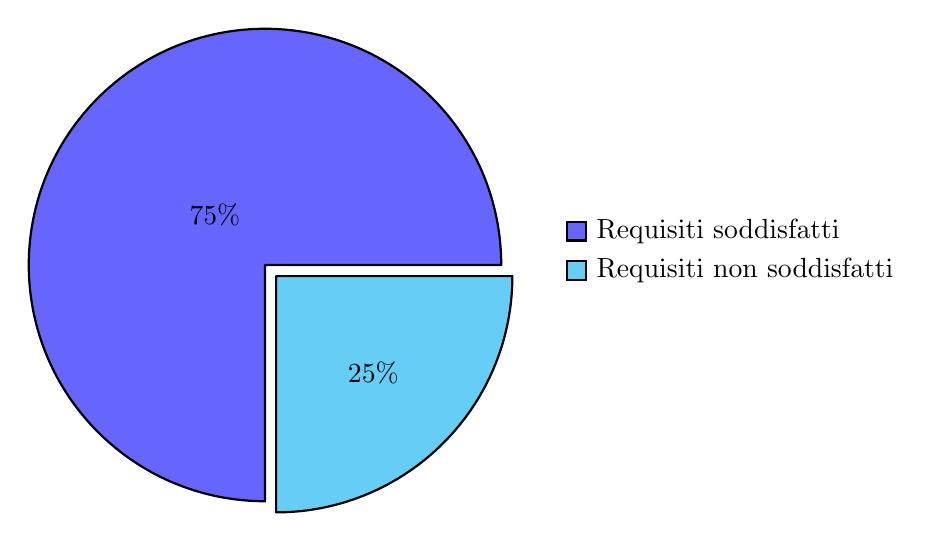
\begin{tikzpicture}
                \pie [explode=0.1, text=legend] { 75/Requisiti soddisfatti, 25/Requisiti non soddisfatti }
                \end{tikzpicture}
                \caption{Percentuale di requisiti funzionali soddisfatti}
        \end{figure}
        \begin{figure}[H]
                \centering
                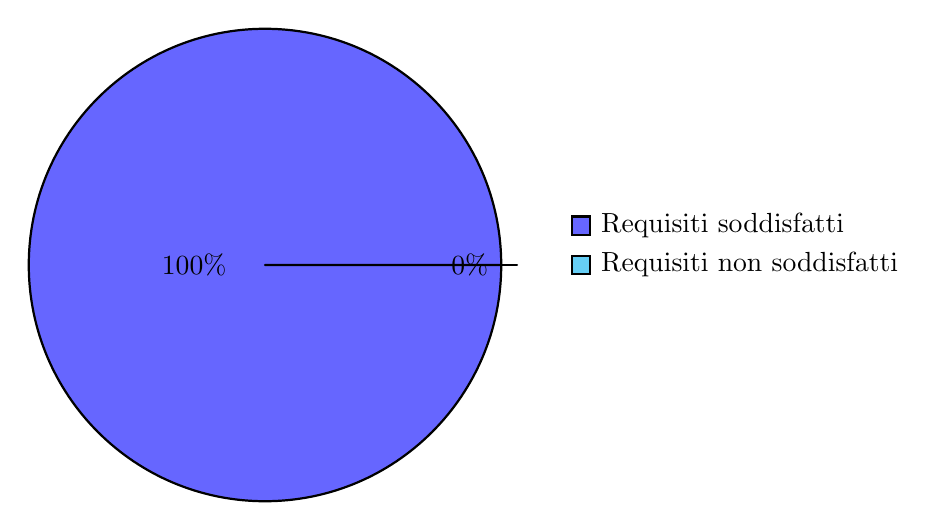
\begin{tikzpicture}
                \pie [explode=0.1, text=legend] { 100/Requisiti soddisfatti, 0/Requisiti non soddisfatti }
                \end{tikzpicture}
                \caption{Percentuale di requisiti funzionali obbligatori soddisfatti}
        \end{figure}
        \begin{figure}[H]
                \centering
                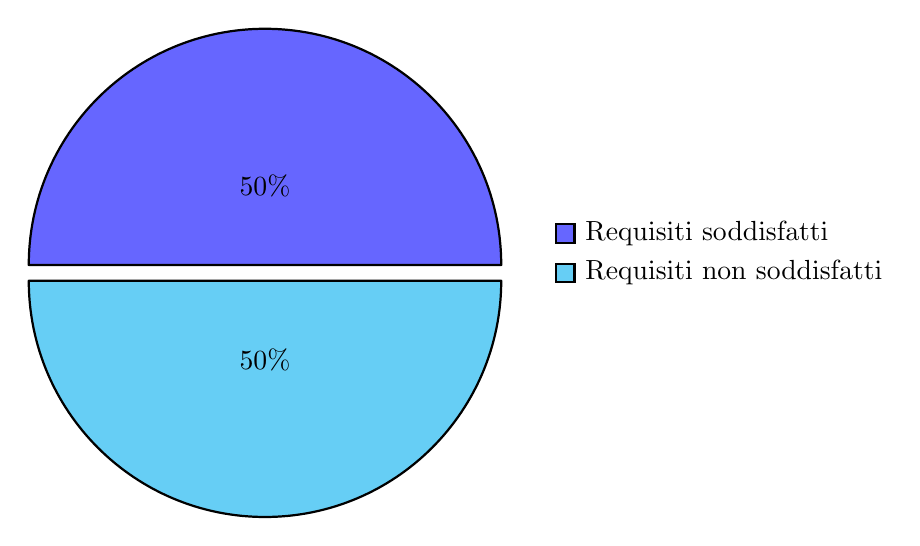
\begin{tikzpicture}
                \pie [explode=0.1, text=legend] { 50/Requisiti soddisfatti, 50/Requisiti non soddisfatti }
                \end{tikzpicture}
                \caption{Percentuale di requisiti funzionali opzionali soddisfatti}
        \end{figure}
        \begin{figure}[H]
                \centering
                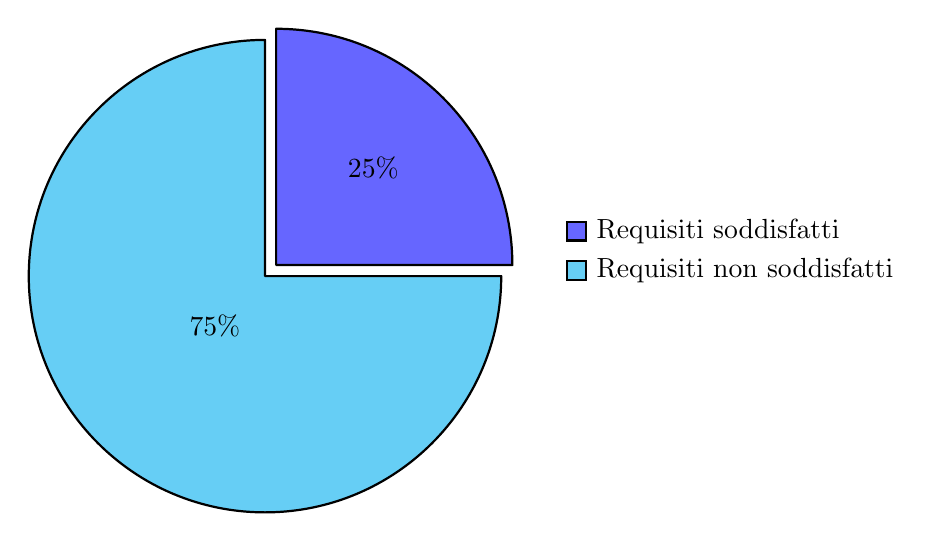
\begin{tikzpicture}
                \pie [explode=0.1, text=legend] { 25/Requisiti soddisfatti, 75/Requisiti non soddisfatti }
                \end{tikzpicture}
                \caption{Percentuale di requisiti funzionali desiderabili soddisfatti}
        \end{figure}
    }
\end{document}
